% Options for packages loaded elsewhere
\PassOptionsToPackage{unicode}{hyperref}
\PassOptionsToPackage{hyphens}{url}
%
\documentclass[
]{book}
\usepackage{amsmath,amssymb}
\usepackage{iftex}
\ifPDFTeX
  \usepackage[T1]{fontenc}
  \usepackage[utf8]{inputenc}
  \usepackage{textcomp} % provide euro and other symbols
\else % if luatex or xetex
  \usepackage{unicode-math} % this also loads fontspec
  \defaultfontfeatures{Scale=MatchLowercase}
  \defaultfontfeatures[\rmfamily]{Ligatures=TeX,Scale=1}
\fi
\usepackage{lmodern}
\ifPDFTeX\else
  % xetex/luatex font selection
\fi
% Use upquote if available, for straight quotes in verbatim environments
\IfFileExists{upquote.sty}{\usepackage{upquote}}{}
\IfFileExists{microtype.sty}{% use microtype if available
  \usepackage[]{microtype}
  \UseMicrotypeSet[protrusion]{basicmath} % disable protrusion for tt fonts
}{}
\makeatletter
\@ifundefined{KOMAClassName}{% if non-KOMA class
  \IfFileExists{parskip.sty}{%
    \usepackage{parskip}
  }{% else
    \setlength{\parindent}{0pt}
    \setlength{\parskip}{6pt plus 2pt minus 1pt}}
}{% if KOMA class
  \KOMAoptions{parskip=half}}
\makeatother
\usepackage{xcolor}
\usepackage{color}
\usepackage{fancyvrb}
\newcommand{\VerbBar}{|}
\newcommand{\VERB}{\Verb[commandchars=\\\{\}]}
\DefineVerbatimEnvironment{Highlighting}{Verbatim}{commandchars=\\\{\}}
% Add ',fontsize=\small' for more characters per line
\usepackage{framed}
\definecolor{shadecolor}{RGB}{248,248,248}
\newenvironment{Shaded}{\begin{snugshade}}{\end{snugshade}}
\newcommand{\AlertTok}[1]{\textcolor[rgb]{0.94,0.16,0.16}{#1}}
\newcommand{\AnnotationTok}[1]{\textcolor[rgb]{0.56,0.35,0.01}{\textbf{\textit{#1}}}}
\newcommand{\AttributeTok}[1]{\textcolor[rgb]{0.13,0.29,0.53}{#1}}
\newcommand{\BaseNTok}[1]{\textcolor[rgb]{0.00,0.00,0.81}{#1}}
\newcommand{\BuiltInTok}[1]{#1}
\newcommand{\CharTok}[1]{\textcolor[rgb]{0.31,0.60,0.02}{#1}}
\newcommand{\CommentTok}[1]{\textcolor[rgb]{0.56,0.35,0.01}{\textit{#1}}}
\newcommand{\CommentVarTok}[1]{\textcolor[rgb]{0.56,0.35,0.01}{\textbf{\textit{#1}}}}
\newcommand{\ConstantTok}[1]{\textcolor[rgb]{0.56,0.35,0.01}{#1}}
\newcommand{\ControlFlowTok}[1]{\textcolor[rgb]{0.13,0.29,0.53}{\textbf{#1}}}
\newcommand{\DataTypeTok}[1]{\textcolor[rgb]{0.13,0.29,0.53}{#1}}
\newcommand{\DecValTok}[1]{\textcolor[rgb]{0.00,0.00,0.81}{#1}}
\newcommand{\DocumentationTok}[1]{\textcolor[rgb]{0.56,0.35,0.01}{\textbf{\textit{#1}}}}
\newcommand{\ErrorTok}[1]{\textcolor[rgb]{0.64,0.00,0.00}{\textbf{#1}}}
\newcommand{\ExtensionTok}[1]{#1}
\newcommand{\FloatTok}[1]{\textcolor[rgb]{0.00,0.00,0.81}{#1}}
\newcommand{\FunctionTok}[1]{\textcolor[rgb]{0.13,0.29,0.53}{\textbf{#1}}}
\newcommand{\ImportTok}[1]{#1}
\newcommand{\InformationTok}[1]{\textcolor[rgb]{0.56,0.35,0.01}{\textbf{\textit{#1}}}}
\newcommand{\KeywordTok}[1]{\textcolor[rgb]{0.13,0.29,0.53}{\textbf{#1}}}
\newcommand{\NormalTok}[1]{#1}
\newcommand{\OperatorTok}[1]{\textcolor[rgb]{0.81,0.36,0.00}{\textbf{#1}}}
\newcommand{\OtherTok}[1]{\textcolor[rgb]{0.56,0.35,0.01}{#1}}
\newcommand{\PreprocessorTok}[1]{\textcolor[rgb]{0.56,0.35,0.01}{\textit{#1}}}
\newcommand{\RegionMarkerTok}[1]{#1}
\newcommand{\SpecialCharTok}[1]{\textcolor[rgb]{0.81,0.36,0.00}{\textbf{#1}}}
\newcommand{\SpecialStringTok}[1]{\textcolor[rgb]{0.31,0.60,0.02}{#1}}
\newcommand{\StringTok}[1]{\textcolor[rgb]{0.31,0.60,0.02}{#1}}
\newcommand{\VariableTok}[1]{\textcolor[rgb]{0.00,0.00,0.00}{#1}}
\newcommand{\VerbatimStringTok}[1]{\textcolor[rgb]{0.31,0.60,0.02}{#1}}
\newcommand{\WarningTok}[1]{\textcolor[rgb]{0.56,0.35,0.01}{\textbf{\textit{#1}}}}
\usepackage{longtable,booktabs,array}
\usepackage{calc} % for calculating minipage widths
% Correct order of tables after \paragraph or \subparagraph
\usepackage{etoolbox}
\makeatletter
\patchcmd\longtable{\par}{\if@noskipsec\mbox{}\fi\par}{}{}
\makeatother
% Allow footnotes in longtable head/foot
\IfFileExists{footnotehyper.sty}{\usepackage{footnotehyper}}{\usepackage{footnote}}
\makesavenoteenv{longtable}
\usepackage{graphicx}
\makeatletter
\def\maxwidth{\ifdim\Gin@nat@width>\linewidth\linewidth\else\Gin@nat@width\fi}
\def\maxheight{\ifdim\Gin@nat@height>\textheight\textheight\else\Gin@nat@height\fi}
\makeatother
% Scale images if necessary, so that they will not overflow the page
% margins by default, and it is still possible to overwrite the defaults
% using explicit options in \includegraphics[width, height, ...]{}
\setkeys{Gin}{width=\maxwidth,height=\maxheight,keepaspectratio}
% Set default figure placement to htbp
\makeatletter
\def\fps@figure{htbp}
\makeatother
\setlength{\emergencystretch}{3em} % prevent overfull lines
\providecommand{\tightlist}{%
  \setlength{\itemsep}{0pt}\setlength{\parskip}{0pt}}
\setcounter{secnumdepth}{5}
\usepackage{booktabs}
\usepackage{amsthm}
\makeatletter
\def\thm@space@setup{%
  \thm@preskip=8pt plus 2pt minus 4pt
  \thm@postskip=\thm@preskip
}
\makeatother
\ifLuaTeX
  \usepackage{selnolig}  % disable illegal ligatures
\fi
\usepackage[]{natbib}
\bibliographystyle{apalike}
\IfFileExists{bookmark.sty}{\usepackage{bookmark}}{\usepackage{hyperref}}
\IfFileExists{xurl.sty}{\usepackage{xurl}}{} % add URL line breaks if available
\urlstyle{same}
\hypersetup{
  pdftitle={Linear Models for Data Science},
  pdfauthor={Jeffrey Woo},
  hidelinks,
  pdfcreator={LaTeX via pandoc}}

\title{Linear Models for Data Science}
\author{Jeffrey Woo}
\date{2025-06-09}

\begin{document}
\maketitle

{
\setcounter{tocdepth}{1}
\tableofcontents
}
\hypertarget{preface}{%
\chapter*{Preface}\label{preface}}
\addcontentsline{toc}{chapter}{Preface}

\hypertarget{who-is-this-book-for}{%
\section*{Who is this book for?}\label{who-is-this-book-for}}
\addcontentsline{toc}{section}{Who is this book for?}

There are many books on linear models, with various expectations for different levels of familiarity with statistical, mathematical, and coding concepts. These books generally fall into one of two camps:

\begin{enumerate}
\def\labelenumi{\arabic{enumi}.}
\tightlist
\item
  Little to no familiarity with statistical and mathematical concepts, but fairly familiar to coding. These books tend to be written for programmers who want to get into data science. These books tend to explain linear models while trying to avoid statistical and mathematical concepts as much as possible. These books tend to present linear models in a recipe format giving readers directions on what to do to build their models.
\end{enumerate}

The drawback of such books is that readers do not get much understanding of the underlying concepts of linear models. It is impossible to give directions covering every possible scenario in the real world as real data are messy. Practitioners of data science often have to think outside the box in order to make linear models work for their particular data, and it is difficult to do so without understanding the mathematical framework of linear models.

\begin{enumerate}
\def\labelenumi{\arabic{enumi}.}
\setcounter{enumi}{1}
\tightlist
\item
  Familiarity with mathematical notation and introductory statistical concepts such as statistical inference, and little to no familiarity with coding. These books tend to be written for mathematicians (or anyone with a strong background in mathematics) who want to get into data science. These books cover the mathematical framework of linear models thoroughly.
\end{enumerate}

The drawback of such books is that readers must be comfortable with mathematical notation. This limits the audience for such books to people with fairly thorough training in mathematics. People without such training will get lost trying to read such books, and do not understand why we need to know the mathematical foundations to use linear models in data science.

This book is meant to be readable by both groups of readers. Some foundational mathematical knowledge will be presented, but will be written so that is readable by anyone. This book will also explain what these knowledge mean in the context of data science. Practical advice, based on the foundational mathematical knowledge, will also be given.

This book accompanies the course STAT 6021: Linear Models for Data Science, for the Masters of Data Science (MSDS) program at the University of Virginia School of Data Science.

As introductory statistics and introductory programming are pre-requisites for entering the MSDS program, this book assumes basic knowledge of statistical inference and coding. Review materials covering these concepts are provided separately for enrolled students.

\hypertarget{chapters}{%
\section*{Chapters}\label{chapters}}
\addcontentsline{toc}{section}{Chapters}

The chapters for the book is as follows:

\begin{itemize}
\item
  Chapters \ref{wrangling} and \ref{viz} focus on core R skills needed: data wrangling and data visualization. These are R skills needed to perform regression analysis.
\item
  Chapters \ref{slr}, \ref{inf}, and \ref{diag} cover simple linear regression (SLR). This is the simplest scenario in regression when we have one predictor and one response variable that is quantitative. We are using this scenario to be able to more clearly explain concepts in regression before moving into the more practical multiple linear regression (MLR), which involves multiple predictors.
\item
  Chapters \ref{mlr} to \ref{out} cover multiple linear regression: when we have multiple predictors and one response variable that is quantitative.
\item
  Chapters \ref{logistic1} and \ref{logistic2} cover logistic regression: when we have a response variable that is binary.
\end{itemize}

\hypertarget{how-to-use-this-book}{%
\section*{How to use this book}\label{how-to-use-this-book}}
\addcontentsline{toc}{section}{How to use this book}

\begin{itemize}
\item
  If you are using the provided R code from each chapter, please remember to clear your R environment whenever you move to a new chapter. This can be done by typing \texttt{rm(list\ =\ ls())}.
\item
  For Chapters \ref{slr} to \ref{logistic2}, there is an R tutorial provided in the last section. You should also clear your R environment before running the code in the tutorials.
\item
  Some additional resources are provided for students enrolled in STAT 6021. These include:

  \begin{itemize}
  \tightlist
  \item
    Learning objectives.
  \item
    Explainer videos.
  \item
    Practice questions.
  \item
    Assignments.
  \end{itemize}
\end{itemize}

\hypertarget{data-sets-used}{%
\section*{Data sets used}\label{data-sets-used}}
\addcontentsline{toc}{section}{Data sets used}

I have tried to use as many open source data sets as much as possible so that readers can work on the various examples I have provided on their own. However, some data sets may not be open source and were shared by other statistics and data science educators over my years of teaching this class (or variations of it) since 2013. It is my goal to eventually use only open source data sets.

\hypertarget{reporting-issues-with-this-book}{%
\section*{Reporting issues with this book}\label{reporting-issues-with-this-book}}
\addcontentsline{toc}{section}{Reporting issues with this book}

This book is mostly a compilation of course notes that were originally written as separate chapters. While effort has been made to fix typos, issues may still exist. If you find any issues (typos, formatting, etc), please report them at \url{https://github.com/jwooSDS/linear_models/issues}. Please be as specific as you can, including providing the specific section and paragraph where the issue is found.

\hypertarget{other-resources}{%
\section*{Other resources}\label{other-resources}}
\addcontentsline{toc}{section}{Other resources}

Some other resources that readers may want to check out:

\begin{itemize}
\item
  \emph{OpenIntro Statistics}, 4th ed.~Diez, Cetinkaya-Rundel, Barr, OpenIntro. Get free PDF version at \url{https://leanpub.com/os}, just set the price that you want to pay to \$0. This is a good book for introductory statistics.
\item
  \emph{Introduction to Probability for Data Science}, Chan. \url{https://probability4datascience.com/index.html}. This book covers the fundamentals of probability and mathematics needed for data science. It does a good job explaining how seemingly abstract mathematical concepts are needed and applied in data science.
\item
  \emph{Linear Models with R}, 2nd ed.~Faraway. This is probably one of the few books that balances between the two camps that I wrote about earlier. It does require familiarity with matrices and linear algebra though.
\item
  \emph{Introduction to Linear Regression Analysis}, 5th or 6th ed.~Montgomery, Peck, Vining. You may be able to access an e-version of the book through your university library if you are affiliated with a university. This book is mathematically rigorous so is useful to those who are interested in mathematical proofs that is not covered.
\item
  \emph{Applied Linear Statistical Models} (ALSM), Kutner, Nachtsheim, Neter, Li, 5th ed.~This book covers a wide range of topics in linear models and is also mathematically rigorous.
\item
  \emph{Applied Linear Regression Models} (ALRM), Kutner, Nachtsheim, Neter, 4th ed.~ALRM is the same as the first 14 chapters of ALSM. The second part of ALSM covers topics in Design of Experiments, which I highly recommend if you are interested in those topics.
\end{itemize}

\hypertarget{slr}{%
\chapter{Basics with Simple Linear Regression (SLR)}\label{slr}}

\hypertarget{introduction-hi}{%
\section{Introduction HI!!!!}\label{introduction-hi}}

We will start this module by introducing the simple linear regression model. Simple linear regression uses the term ``simple,'' because it concerns the study of only one predictor variable with one quantitative response variable. In contrast, multiple linear regression, which we will study in future modules, uses the term ``multiple,'' because it concerns the study of two or more predictor variables with one quantitative response variable. We start with simple linear regression as it is much easier to visualize concepts in regression models when there is only one predictor variable.

For the time being, we will only consider predictor variables that are quantitative. We will consider predictor variables that are categorical in future modules.

The most common way of visualizing the relationship between one quantitative predictor variable and one quantitative response variable is with a scatter plot. In the simulated example below, we have data from 6000 UVa undergraduate students on the amount of time they spend studying in a week (in minutes), and how many courses they are taking in the semester (3 or 4 credit courses).

\begin{Shaded}
\begin{Highlighting}[]
\DocumentationTok{\#\#create dataframe}
\NormalTok{df}\OtherTok{\textless{}{-}}\FunctionTok{data.frame}\NormalTok{(study,courses)}

\DocumentationTok{\#\#fit regression}
\NormalTok{result}\OtherTok{\textless{}{-}}\FunctionTok{lm}\NormalTok{(study}\SpecialCharTok{\textasciitilde{}}\NormalTok{courses, }\AttributeTok{data=}\NormalTok{df)}
\end{Highlighting}
\end{Shaded}

\begin{Shaded}
\begin{Highlighting}[]
\DocumentationTok{\#\#create scatterplot with regression line overlaid}
\FunctionTok{plot}\NormalTok{(df}\SpecialCharTok{$}\NormalTok{courses, df}\SpecialCharTok{$}\NormalTok{study, }\AttributeTok{xlab=}\StringTok{"\# of Courses"}\NormalTok{, }\AttributeTok{ylab=}\StringTok{"Study Time (Mins)"}\NormalTok{)}
\FunctionTok{abline}\NormalTok{(result)}
\end{Highlighting}
\end{Shaded}

\begin{figure}
\centering
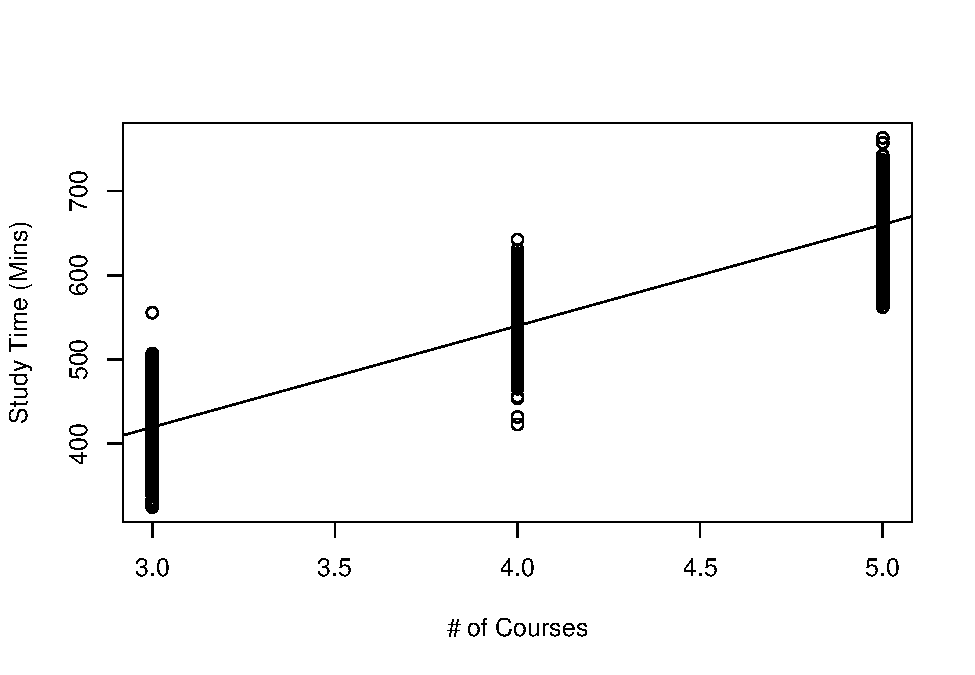
\includegraphics{bookdown-demo_files/figure-latex/scatter-courses-1.pdf}
\caption{\label{fig:scatter-courses}Scatterplot of Study Time against Number of Courses Taken}
\end{figure}

Questions that we may have include:

\begin{itemize}
\tightlist
\item
  Are study time and the number of courses taken related to one another?
\item
  How strong is this relationship?
\item
  Could we use the data to make a prediction for the study time of a student who is not in this scatterplot?
\item
  How confident are we of the prediction?
\end{itemize}

These questions can be answered using simple linear regression.

Note that we will only be learning about models with just one response variable. We will not cover multivariate regression, which is used when there is more than one response variable. There may be some confusion between ``multiple'' linear regression and ``multivariate'' regression due to the closeness in terminology.

\hypertarget{basic-ideas-with-statistics}{%
\subsection{Basic Ideas with Statistics}\label{basic-ideas-with-statistics}}

\hypertarget{population-vs-sample}{%
\subsubsection{Population vs Sample}\label{population-vs-sample}}

Statistical methods are usually used to make inferences about the \textbf{population} based on information from a \textbf{sample}.

\begin{itemize}
\tightlist
\item
  A sample is the collection of units that is actually measured or surveyed in a study.
\item
  The population includes all units of interest.
\end{itemize}

In the study time example above, the population is all UVa undergraduate students, while the sample is the 6000 students that we have data on and are displayed on the scatterplot.

\hypertarget{parameters-vs-statistics}{%
\subsubsection{Parameters vs Statistics}\label{parameters-vs-statistics}}

\begin{itemize}
\tightlist
\item
  \textbf{Parameters} are numerical quantities that describe a population.
\item
  \textbf{Statistics} are numerical quantities that describe a sample.
\end{itemize}

In the study time example, an example of a parameter will be the average study time among all UVa undergraduate students (called the population mean), and an example of a statistic will be the average study time among the 6000 UVa students we have data on (called the sample mean).

Notice that in real life, we will rarely know the actual numerical value of a parameter. So we use the numerical value of the statistic to \textbf{estimate} the unknown numerical value of the corresponding parameter.

We also have different notation for parameters and statistics. For example,

\begin{itemize}
\tightlist
\item
  the population mean is denoted as \(\mu\).
\item
  the sample mean is denoted as \(\bar{x}\).
\end{itemize}

We say that \(\bar{x}\) is an \textbf{estimator} of \(\mu\).

It is important to pay attention to whether we are describing a statistic (a known value that can be calculated) or a parameter (an unknown value).

\hypertarget{motivation}{%
\subsection{Motivation}\label{motivation}}

Linear regression models generally have two primary uses:

\begin{enumerate}
\def\labelenumi{\arabic{enumi}.}
\tightlist
\item
  \textbf{Prediction}: Predict a future value of a response variable, using information from predictor variables.
\item
  \textbf{Association}: Quantify the relationship between variables. How does a change in the predictor variable change the value of the response variable?
\end{enumerate}

We always distinguish between a \textbf{response variable, denoted by \(y\)}, and a \textbf{predictor variable, denoted by \(x\)}. In most statistical models, we say that the response variable can be approximated by some \textbf{mathematical function, denoted by \(f\)}, of the predictor variable, i.e.

\[
y \approx f(x).
\]
Oftentimes, we write this relationship as

\[
y = f(x) + \epsilon,
\]

where \textbf{\(\epsilon\) denotes a random error term}, with a mean of 0. The error term cannot be predicted based on the data we have.

There are various statistical methods to estimate \(f\). Once we estimate \(f\), we can use our method for prediction and / or association.

Using the study time example above:

\begin{itemize}
\tightlist
\item
  a prediction example: a student intends to take 4 courses in the semester. What is this student's predicted study time, on average?
\item
  an association example: we want to see how taking more courses increases study time.
\end{itemize}

\hypertarget{practice-questions}{%
\subsubsection{Practice questions}\label{practice-questions}}

In the examples below, are we using a regression model for prediction or for association?

\begin{enumerate}
\def\labelenumi{\arabic{enumi}.}
\item
  It is early in the morning and I am heading out for the rest of the day. I want to know the weather forecast for the rest of the day so I know what to wear.
\item
  An executive for a sports league wants to assess how increasing the length of commercial breaks may impact the enjoyment of sports fans who watch games on TV.
\item
  The Education Secretary would like to evaluate how certain factors such as use of technology in classrooms and investment in teacher training and teacher pay are associated with reading skills of students.
\item
  When buying a home, the prospective buyer would like to know if the home is under- or over- priced, given its characteristics.
\end{enumerate}

\hypertarget{simple-linear-regression-slr}{%
\section{Simple Linear Regression (SLR)}\label{simple-linear-regression-slr}}

In simple linear regression (SLR), the function \(f\) that relates the predictor variable with the response variable is typically \(\beta_0 + \beta_1 x\). Mathematically, we express this as

\[
y \approx \beta_0 + \beta_1 x,
\]

or in other words, that the response variable has an approximately linear relationship with the predictor variable.

In SLR, this relationship is more explicitly formulated as the \textbf{simple linear regression equation}:

\begin{equation} 
E(y|x)=\beta_0+\beta_{1}x.
\label{eq:SLR}
\end{equation}

\begin{itemize}
\item
  \(\beta_0\) and \(\beta_1\) are parameters in the SLR equation, and we want to estimate them.
\item
  These parameters are sometimes called \textbf{regression coefficients}.
\item
  \(\beta_1\) is also called the \textbf{slope. It denotes the change in \(y\), on average, when \(x\) increases by one unit.}
\item
  \(\beta_0\) is also called the \textbf{intercept. It denotes the average of \(y\) when \(x=0\).}
\item
  The notation on the left hand side of \eqref{eq:SLR} denotes the \textbf{expected value} of the response variable, for a fixed value of the predictor variable. What \eqref{eq:SLR} implies is that, for each value of the predictor variable \(x\), the expected value of the response variable \(y\) is \(\beta_0+\beta_{1}x\). The expected value is also the population mean. Applying \eqref{eq:SLR} to our study time example, it implies that:

  \begin{itemize}
  \tightlist
  \item
    for students who take 3 courses, their expected study time is equal to \(\beta_0 + 3\beta_1\),
  \item
    for students who take 4 courses, their expected study time is equal to \(\beta_0 + 4\beta_1\),
  \item
    for students who take 5 courses, their expected study time is equal to \(\beta_0 + 5\beta_1\).
  \end{itemize}
\end{itemize}

So \(f(x) = \beta_0 + \beta_1x\) gives us the value of the expected value of the response variable for a specific value of the predictor variable. But, for each value of the predictor variable, the value of the response variable is not a constant. We say that for each value of \(x\), the response variable \(y\) has some variance. The variance of the response variable for each value of \(x\) is the same as the variance of the error term, \(\epsilon\). Thus we have the \textbf{simple linear regression model}

\begin{equation} 
y=\beta_0+\beta_{1} x + \epsilon. 
\label{eq:SLRmod}
\end{equation}

We need to make some assumptions for the error term \(\epsilon\). Generally, the assumptions are:

\begin{enumerate}
\def\labelenumi{\arabic{enumi}.}
\tightlist
\item
  The errors have mean 0.
\item
  The \textbf{errors have variance denoted by \(\sigma^2\)}. Notice this variance is constant.
\item
  The errors are independent.
\item
  The errors are normally distributed.
\end{enumerate}

From \eqref{eq:SLRmod}, notice we have another parameter, \(\sigma^2\).

We will go into more detail about what these assumptions mean, and how to assess whether they are met, in module \ref{diag}.

What these assumptions mean is that for each value of the predictor variable \(x\), the response variable:

\begin{enumerate}
\def\labelenumi{\arabic{enumi}.}
\tightlist
\item
  follows a normal distribution,
\item
  with mean equal to \(\beta_0+\beta_{1} x\),
\item
  and variance equal to \(\sigma^2\).
\end{enumerate}

Using our study time example, it means that:

\begin{itemize}
\tightlist
\item
  for students who take 3 courses, the distribution of their study times is \(N(\beta_0 + 3\beta_1, \sigma^2)\).
\item
  for students who take 4 courses, the distribution of their study times is \(N(\beta_0 + 4\beta_1, \sigma^2)\).
\item
  for students who take 5 courses, the distribution of their study times is \(N(\beta_0 + 5\beta_1, \sigma^2)\).
\end{itemize}

So if we were to subset our dataframe into three subsets, one with students who take 3 courses, another subset for students who take 4 courses, and another subset for students who take 5 courses, and then create a density plot of study times for each subset, each density plot should follow a normal distribution, with different means, and the same spread.

Let us take a look at these density plots next.

\begin{Shaded}
\begin{Highlighting}[]
\FunctionTok{library}\NormalTok{(tidyverse)}
\end{Highlighting}
\end{Shaded}

\begin{Shaded}
\begin{Highlighting}[]
\DocumentationTok{\#\#subset dataframe}
\NormalTok{x}\FloatTok{.3}\OtherTok{\textless{}{-}}\NormalTok{df[}\FunctionTok{which}\NormalTok{(df}\SpecialCharTok{$}\NormalTok{courses}\SpecialCharTok{==}\DecValTok{3}\NormalTok{),]}
\DocumentationTok{\#\#density plot of study time for students taking 3 courses}
\FunctionTok{ggplot}\NormalTok{(x}\FloatTok{.3}\NormalTok{,}\FunctionTok{aes}\NormalTok{(}\AttributeTok{x=}\NormalTok{study))}\SpecialCharTok{+}
  \FunctionTok{geom\_density}\NormalTok{()}\SpecialCharTok{+}
  \FunctionTok{labs}\NormalTok{(}\AttributeTok{x=}\StringTok{"Study Time (Mins)"}\NormalTok{, }\AttributeTok{title=}\StringTok{"Dist of Study Times with 3 Courses"}\NormalTok{)}
\end{Highlighting}
\end{Shaded}

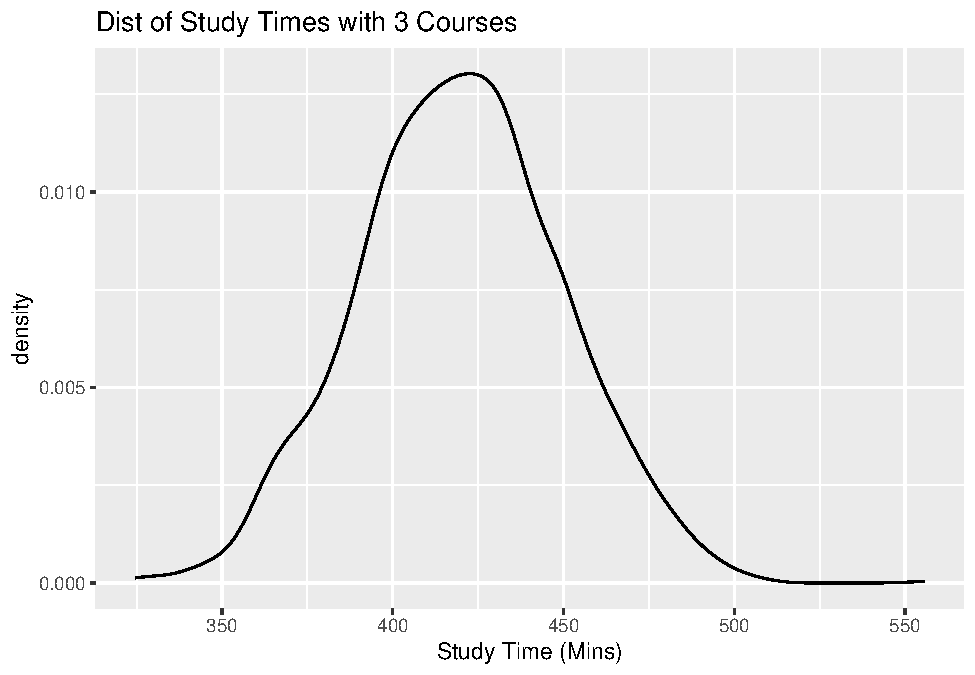
\includegraphics{bookdown-demo_files/figure-latex/unnamed-chunk-5-1.pdf}

\begin{Shaded}
\begin{Highlighting}[]
\DocumentationTok{\#\#subset dataframe}
\NormalTok{x}\FloatTok{.4}\OtherTok{\textless{}{-}}\NormalTok{df[}\FunctionTok{which}\NormalTok{(df}\SpecialCharTok{$}\NormalTok{courses}\SpecialCharTok{==}\DecValTok{4}\NormalTok{),]}
\DocumentationTok{\#\#density plot of study time for students taking 4 courses}
\FunctionTok{ggplot}\NormalTok{(x}\FloatTok{.4}\NormalTok{,}\FunctionTok{aes}\NormalTok{(}\AttributeTok{x=}\NormalTok{study))}\SpecialCharTok{+}
  \FunctionTok{geom\_density}\NormalTok{()}\SpecialCharTok{+}
  \FunctionTok{labs}\NormalTok{(}\AttributeTok{x=}\StringTok{"Study Time (Mins)"}\NormalTok{, }\AttributeTok{title=}\StringTok{"Dist of Study Times with 4 Courses"}\NormalTok{)}
\end{Highlighting}
\end{Shaded}

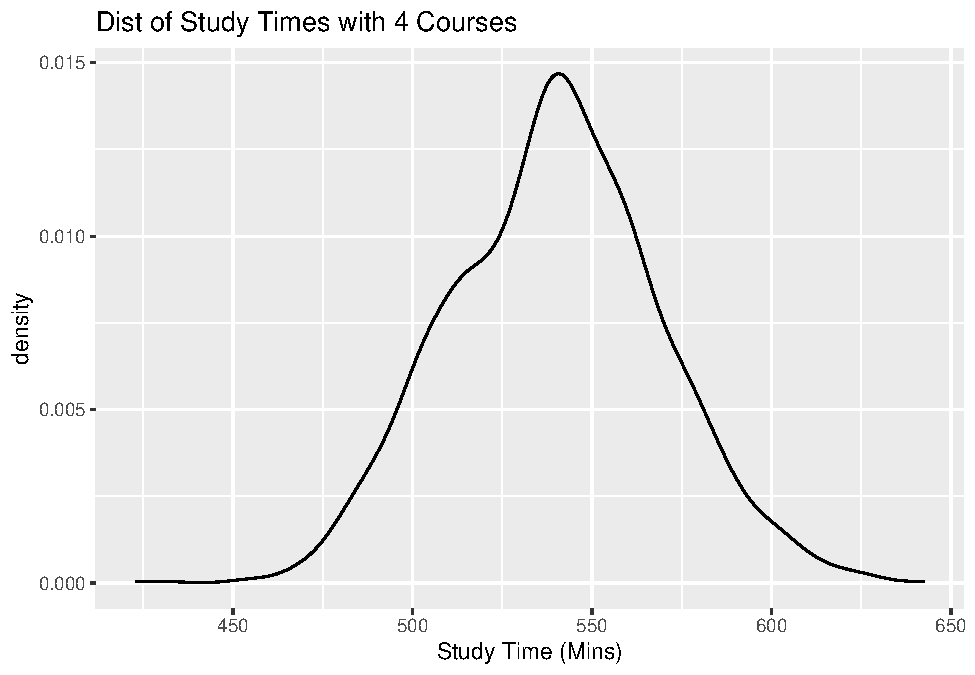
\includegraphics{bookdown-demo_files/figure-latex/unnamed-chunk-5-2.pdf}

\begin{Shaded}
\begin{Highlighting}[]
\DocumentationTok{\#\#subset dataframe}
\NormalTok{x}\FloatTok{.5}\OtherTok{\textless{}{-}}\NormalTok{df[}\FunctionTok{which}\NormalTok{(df}\SpecialCharTok{$}\NormalTok{courses}\SpecialCharTok{==}\DecValTok{5}\NormalTok{),]}
\DocumentationTok{\#\#density plot of study time for students taking 5 courses}
\FunctionTok{ggplot}\NormalTok{(x}\FloatTok{.5}\NormalTok{,}\FunctionTok{aes}\NormalTok{(}\AttributeTok{x=}\NormalTok{study))}\SpecialCharTok{+}
  \FunctionTok{geom\_density}\NormalTok{()}\SpecialCharTok{+}
  \FunctionTok{labs}\NormalTok{(}\AttributeTok{x=}\StringTok{"Study Time (Mins)"}\NormalTok{, }\AttributeTok{title=}\StringTok{"Dist of Study Times with 5 Courses"}\NormalTok{)}
\end{Highlighting}
\end{Shaded}

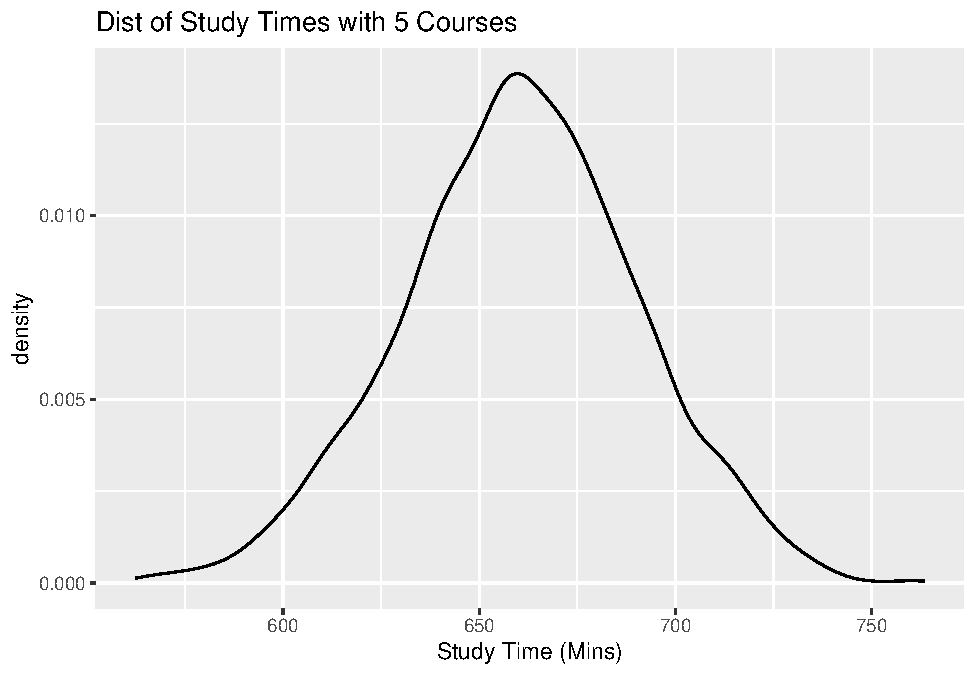
\includegraphics{bookdown-demo_files/figure-latex/unnamed-chunk-5-3.pdf}

Notice all of these plots are normal, with different means (centers), and similar spreads.

\emph{Please see the associated video for more explanation about the distribution of the response variable, for each value of the predictor variable, in an SLR setting.}

\hypertarget{estimating-regression-coefficients-in-slr}{%
\section{Estimating Regression Coefficients in SLR}\label{estimating-regression-coefficients-in-slr}}

From \eqref{eq:SLR} and \eqref{eq:SLRmod}, we noted that we have to estimate the regression coefficients \(\beta_0, \beta_1\) as well as the parameter \(\sigma^2\) associated with the error term. As mentioned earlier, we are unable to obtain numerical values of these parameters as we do not have data from the entire population. So what we do is use the data from our sample to estimate these parameters.

We estimate \(\beta_0,\beta_1\) using \(\hat{\beta}_0,\hat{\beta}_1\) based on a sample of observations \((x_i,y_i)\) of size \(n\).

The subscripts associated with the response and predictor variables denote which data point that value belongs to. Let us take a look at the first few rows of the data frame for the study time example:

\begin{Shaded}
\begin{Highlighting}[]
\FunctionTok{head}\NormalTok{(df)}
\end{Highlighting}
\end{Shaded}

\begin{verbatim}
##      study courses
## 1 429.8311       3
## 2 458.4588       3
## 3 391.9406       3
## 4 378.0196       3
## 5 397.9856       3
## 6 405.7145       3
\end{verbatim}

For example, \(x_1\) denotes the number of courses taken by student number 1 in the dataframe, which is 3. \(y_4\) denotes the study time for student number 4 in the dataframe, which is 378.0196456.

Following \eqref{eq:SLR} and \eqref{eq:SLRmod}, the sample versions are

\begin{equation} 
\hat{y}=\hat{\beta}_0+\hat{\beta}_1 x
\label{eq:fitted}
\end{equation}

and

\begin{equation} 
y=\hat{\beta}_0+\hat{\beta}_1 x + e
\label{eq:fitted-model}
\end{equation}

respectively. \eqref{eq:fitted} is called the \textbf{estimated SLR equation}, or \textbf{fitted SLR equation}. \eqref{eq:fitted-model} is called the \textbf{estimated SLR model}.

\(\hat{\beta}_1,\hat{\beta}_0\) are the estimators for \(\beta_1,\beta_0\) respectively. These estimators can be interpreted in the following manner:

\begin{itemize}
\tightlist
\item
  \textbf{\(\hat{\beta}_1\) denotes the change in the predicted \(y\) when \(x\) increases by 1 unit. Alternatively, it denotes the change in \(y\), on average, when \(x\) increases by 1 unit.}
\item
  \textbf{\(\hat{\beta}_0\) denotes the predicted \(y\) when \(x=0\). Alternatively, it denotes the average of \(y\) when \(x=0\).}
\end{itemize}

From \eqref{eq:fitted-model}, notice we use \textbf{\(e\) to denote the residual}, or in other words, the ``error'' in the sample.

From \eqref{eq:fitted} and \eqref{eq:fitted-model}, we have the following quantities that we can compute:

\begin{equation}
\text{Predicted/Fitted values: } \hat{y}_i = \hat{\beta}_0+\hat{\beta}_1 x_i.
\label{eq:fits}
\end{equation}

\begin{equation} 
\text{Residuals: } e_i = y_i-\hat{y}_i.
\label{eq:res}
\end{equation}

\begin{equation} 
\text{Sum of Squared Residuals: } SS_{res} =  \sum\limits_{i=1}^n(y_i-\hat{y}_i)^2.
\label{eq:SSres}
\end{equation}

We compute the estimated coefficients \(\hat{\beta}_1,\hat{\beta}_0\) using the \textbf{method of least squares}, i.e.~choose the numerical values of \(\hat{\beta}_1,\hat{\beta}_0\) that minimize \(SS_{res}\) as given in \eqref{eq:SSres}.

By minimizing \(SS_{res}\) with respect to \(\hat{\beta}_0\) and \(\hat{\beta}_1\), the estimated coefficients in the simple linear regression equation are

\begin{equation} 
\hat{\beta}_1 = \frac{\sum\limits_{i=1}^n(x_i-\bar{x})(y_i-\bar{y})}{\sum\limits_{i=1}^n(x_i-\bar{x})^2}
\label{eq:b1}
\end{equation}

and

\begin{equation} 
\hat{\beta}_0 = \bar{y}- \hat{\beta}_1 \bar{x}
\label{eq:b0}
\end{equation}

\(\hat{\beta}_1, \hat{\beta}_0\) are called \textbf{least squares estimators}.

The minimization of \(SS_{res}\) with respect to \(\hat{\beta}_0\) and \(\hat{\beta}_1\) is done by taking the partial derivatives of \eqref{eq:SSres} with respect to \(\hat{\beta}_1\) and \(\hat{\beta}_0\), setting these two partial derivatives equal to 0, and solving these two equations for \(\hat{\beta}_1\) and \(\hat{\beta}_0\).

Let's take a look at the estimated coefficients for our study time example:

\begin{Shaded}
\begin{Highlighting}[]
\DocumentationTok{\#\#fit regression}
\NormalTok{result}\OtherTok{\textless{}{-}}\FunctionTok{lm}\NormalTok{(study}\SpecialCharTok{\textasciitilde{}}\NormalTok{courses, }\AttributeTok{data=}\NormalTok{df)}
\DocumentationTok{\#\#print out the estimated coefficients}
\NormalTok{result}
\end{Highlighting}
\end{Shaded}

\begin{verbatim}
## 
## Call:
## lm(formula = study ~ courses, data = df)
## 
## Coefficients:
## (Intercept)      courses  
##       58.45       120.39
\end{verbatim}

From our sample of 6000 students, we have

\begin{itemize}
\tightlist
\item
  \(\hat{\beta}_1\) = 120.3930985. The predicted study time increases by 120.3930985 minutes for each additional course taken.
\item
  \(\hat{\beta}_0\) = 58.4482853. The predicted study time is 58.4482853 when no courses are taken. Notice this value does not make sense, as a student cannot be taking 0 courses. If you look at our data, the number of courses taken is 3, 4, or 5. So we should only use our regression when \(3 \leq x \leq 5\). We cannot use it for values of \(x\) outside the range of our data. Making predictions of the response variable for predictors outside the range of the data is called \textbf{extrapolation} and should not be done.
\end{itemize}

\hypertarget{estimating-variance-of-errors-in-slr}{%
\section{Estimating Variance of Errors in SLR}\label{estimating-variance-of-errors-in-slr}}

The estimator of \(\sigma^2\), the variance of the error terms (also the variance of the probability distribution of \(y\) given \(x\)) is
\begin{equation} 
s^2 = MS_{res} = \frac{SS_{res}}{n-2} = \frac{\sum\limits_{i=1}^n e_i^2}{n-2},
\label{eq:variance}
\end{equation}

where \(MS_{res}\) is the called the \textbf{mean squared residuals}.

\(\sigma^2\), the variance of the error terms, measures the spread of the response variable, for each value of \(x\). The smaller this is, the closer the data points are to the regression equation.

\hypertarget{practice-questions-1}{%
\subsection{Practice questions}\label{practice-questions-1}}

Take a look at the scatterplot of study time against number of courses taken, Figure \ref{fig:scatter-courses}. On this plot, label the following:

\begin{itemize}
\tightlist
\item
  estimated SLR equation
\item
  the fitted value when \(x=3\), \(x=4\), and \(x=5\).
\item
  the residual for any data point on the plot of your choosing.
\end{itemize}

\emph{Try these on your own first, then view the associated video to see if you labeled the plot correctly!}

\hypertarget{assessing-linear-association}{%
\section{Assessing Linear Association}\label{assessing-linear-association}}

As noted earlier, the variance of the error terms inform us how close the data points are to the estimated SLR equation. The smaller the variance of the error terms, the closer the data points are to the estimated SLR equation. This in turn implies the linear relationship between the variables is stronger.

We will learn about some common measures that are used to quantify the strength of the linear relationship between the response and predictor variables. Before we do that, we need to define some other terms.

\hypertarget{sum-of-squares}{%
\subsection{Sum of squares}\label{sum-of-squares}}

\begin{equation} 
\text{Total Sum of Squares: } SS_T = \sum\limits_{i=1}^{n} (y_i - \bar{y})^{2}.
\label{eq:SST}
\end{equation}

Total sum of squares is defined as the \textbf{total variance in the response variable}. The larger this value is, the larger the spread is of the response variable.

\begin{equation} 
\text{Regression sum of squares: } SS_R = \sum\limits_{i=1}^{n} (\hat{y_i} - \bar{y})^{2}.
\label{eq:SSR}
\end{equation}

Regression sum of squares is defined as the \textbf{variance in the response variable that can be explained by our regression}.

We also have residual sum of squares, \(SS_{res}\). Its mathematical formulation is given in \eqref{eq:SSres}. It is defined as the \textbf{variance in the response variable that cannot be explained by our regression}.

It can be shown that

\begin{equation}
SS_T = SS_R + SS_{res}.
\label{eq:SS}
\end{equation}

Each of the sums of squares has its associated \textbf{degrees of freedom (df)}:

\begin{itemize}
\tightlist
\item
  df for \(SS_R\): \(df_R = 1\)
\item
  df for \(SS_{res}\): \(df_{res} = n-2\)
\item
  df for \(SS_T\): \(df_T = n-1\)
\end{itemize}

\emph{Please see the associated video for more explanation about the concept behind degrees of freedom.}

\hypertarget{anova-table}{%
\subsection{ANOVA Table}\label{anova-table}}

Information regarding the sums of squares is usually presented in the form of an \textbf{ANOVA (analysis of variance) table}:

\begin{longtable}[]{@{}
  >{\centering\arraybackslash}p{(\columnwidth - 8\tabcolsep) * \real{0.2353}}
  >{\centering\arraybackslash}p{(\columnwidth - 8\tabcolsep) * \real{0.2941}}
  >{\centering\arraybackslash}p{(\columnwidth - 8\tabcolsep) * \real{0.1569}}
  >{\centering\arraybackslash}p{(\columnwidth - 8\tabcolsep) * \real{0.1569}}
  >{\centering\arraybackslash}p{(\columnwidth - 8\tabcolsep) * \real{0.1569}}@{}}
\toprule\noalign{}
\begin{minipage}[b]{\linewidth}\centering
Source of Variation
\end{minipage} & \begin{minipage}[b]{\linewidth}\centering
SS
\end{minipage} & \begin{minipage}[b]{\linewidth}\centering
df
\end{minipage} & \begin{minipage}[b]{\linewidth}\centering
MS
\end{minipage} & \begin{minipage}[b]{\linewidth}\centering
F
\end{minipage} \\
\midrule\noalign{}
\endhead
\bottomrule\noalign{}
\endlastfoot
Regression & \(SS_R=\sum\left(\hat{y_i}-\bar{y}\right)^2\) & \(df_R = 1\) & \(MS_R=\frac{SS_R}{df_R}\) & \(\frac{MS_R}{MS_{res}}\) \\
Error & \(SS_{res} = \sum\left(y_i-\hat{y_i}\right)^2\) & \(df_{res} = n-2\) & \(MS_{res}=\frac{SS_{res}}{df_{res}}\) & \texttt{***} \\
Total & \(SS_T=\sum\left(y_i-\bar{y}\right)^2\) & \(df_T = n-1\) & \texttt{***} & \texttt{***} \\
\end{longtable}

Note:

\begin{itemize}
\tightlist
\item
  Dividing each sum of square with its corresponding degrees of freedom gives the corresponding mean square.
\item
  In the last column, we report an \(F\) statistic, which equal to \(\frac{MS_R}{MS_{res}}\). This \(F\) statistic is associated with an \textbf{ANOVA F test}, which we will look at in more detail in the next subsection.
\end{itemize}

To obtain the ANOVA table for our study time example:

\begin{Shaded}
\begin{Highlighting}[]
\FunctionTok{anova}\NormalTok{(result)}
\end{Highlighting}
\end{Shaded}

\begin{verbatim}
## Analysis of Variance Table
## 
## Response: study
##             Df   Sum Sq  Mean Sq F value    Pr(>F)    
## courses      1 57977993 57977993   65404 < 2.2e-16 ***
## Residuals 5998  5317017      886                      
## ---
## Signif. codes:  0 '***' 0.001 '**' 0.01 '*' 0.05 '.' 0.1 ' ' 1
\end{verbatim}

Notice that R does not print out the information for the line regarding \(SS_T\).

\hypertarget{anova-f-test}{%
\subsection{\texorpdfstring{ANOVA \(F\) Test}{ANOVA F Test}}\label{anova-f-test}}

In SLR, the ANOVA \(F\) statistic from the ANOVA table can be used to test if the slope of the SLR equation is 0 or not. In words, this means that whether there is a linear association between the variables or not. If the slope is 0, it means that changes in the value of the predictor variable do not change the value of the response variable, on average; hence the variables are not linearly associated.

The null and alternative hypotheses are:

\[
H_0: \beta_1 = 0, H_a: \beta_1 \neq 0.
\]
The test statistic is

\begin{equation} 
F = \frac{MS_R}{MS_{res}}
\label{eq:ANOVA}
\end{equation}

and is compared with an \(F_{1,n-2}\) distribution. Note that \(F_{1,n-2}\) is read as an \textbf{F distribution with 1 and \(n-2\) degrees of freedom}.

Going back to the study time example, the \(F\) statistic is \ensuremath{6.5403586\times 10^{4}}. The critical value can be found using

\begin{Shaded}
\begin{Highlighting}[]
\FunctionTok{qf}\NormalTok{(}\DecValTok{1}\FloatTok{{-}0.05}\NormalTok{, }\DecValTok{1}\NormalTok{, }\DecValTok{6000{-}2}\NormalTok{)}
\end{Highlighting}
\end{Shaded}

\begin{verbatim}
## [1] 3.84301
\end{verbatim}

Since our test statistic is larger than the critical value, we reject the null hypothesis. Our data support the claim that the slope is different from 0, or in other words, that there is a linear association between study time and number of courses taken.

\hypertarget{coefficient-of-determination}{%
\subsection{Coefficient of determination}\label{coefficient-of-determination}}

The \textbf{coefficient of determination, \(R^2\),} is

\begin{equation}
R^{2} = \frac{SS_R}{SS_T} = 1 - \frac{SS_{res}}{SS_T}.
\label{eq:R2}
\end{equation}

\(R^{2}\) is an indication of how well the data fits our model. In the context of simple linear regression, it denotes \textbf{the proportion of variance in the response variable that is explained by the predictor}.

A few notes about \(R^2\):

\begin{itemize}
\tightlist
\item
  \(0 \leq R^2 \leq 1\).
\item
  Values closer to 1 indicate a better fit; values closer to 0 indicate a poorer fit.
\item
  Sometimes reported as a percentage.
\end{itemize}

To obtain \(R^2\) for our study time example:

\begin{Shaded}
\begin{Highlighting}[]
\NormalTok{anova.tab}\OtherTok{\textless{}{-}}\FunctionTok{anova}\NormalTok{(result)}
\DocumentationTok{\#\#SST not provided, so we add up SSR and SSres}
\NormalTok{SST}\OtherTok{\textless{}{-}}\FunctionTok{sum}\NormalTok{(anova.tab}\SpecialCharTok{$}\StringTok{"Sum Sq"}\NormalTok{)}
\DocumentationTok{\#\#R2}
\NormalTok{anova.tab}\SpecialCharTok{$}\StringTok{"Sum Sq"}\NormalTok{[}\DecValTok{1}\NormalTok{]}\SpecialCharTok{/}\NormalTok{SST}
\end{Highlighting}
\end{Shaded}

\begin{verbatim}
## [1] 0.9159963
\end{verbatim}

This implies that the proportion of variance in study time that can be explained by the number of courses taken is 0.9159963.

\hypertarget{correlation}{%
\subsection{Correlation}\label{correlation}}

A measure used to quantify the strength of the linear association between two quantitative variables is the \textbf{sample correlation}. The sample correlation, \(\mbox{Corr}(x,y)\) or \(r\), is given by

\begin{equation} 
r = \frac{\sum\limits_{i=1}^{n}(x_i - \bar{x})(y_i - \bar{y})}{\sqrt{\sum\limits_{i=1}^{n}(x_i - \bar{x})^{2}(y_i - \bar{y})^{2}}}.
\label{eq:corr}
\end{equation}

A few notes about \(r\):

\begin{itemize}
\tightlist
\item
  \(-1 \leq r \leq 1\).
\item
  Sign of correlation indicates direction of association. A positive value indicates a positive linear association: as the predictor variable increases, so does the response variable, on average. A negative value indicates a negative linear association: as the predictor variable increases, the response variable decreases, on average.
\item
  Values closer to 1 or -1 indicate a stronger linear association; values closer to 0 indicate a weaker linear association.
\item
  In SLR, it turns out that \(r^2 = R^2\).
\end{itemize}

Using our study time example, the correlation between study time and number of courses taken is

\begin{Shaded}
\begin{Highlighting}[]
\FunctionTok{cor}\NormalTok{(df}\SpecialCharTok{$}\NormalTok{study, df}\SpecialCharTok{$}\NormalTok{courses)}
\end{Highlighting}
\end{Shaded}

\begin{verbatim}
## [1] 0.9570769
\end{verbatim}

This value indicates a very strong and positive linear association between study time and number of courses taken (remember that this is simulated data and is not real).

\hypertarget{how-strong-is-strong}{%
\subsubsection{How strong is strong?}\label{how-strong-is-strong}}

A question that is often raised is how large should the magnitude of the sample correlation be for it to be considered strong? The answer is: it depends on the context. If you are conducting an experiment that is governed by scientific laws (e.g an experiment verifying Newton's 2nd law that \(F = ma\)), we should expect an extremely high correlation. A correlation of 0.9 in such an instance may be considered weak. The value of the correlation you have should be compared with correlations from similar studies in that domain to determine if it is strong or not.

\hypertarget{a-word-of-caution}{%
\section{A Word of Caution}\label{a-word-of-caution}}

To be able to use the measures we have learned (such as correlation, \(R^2\)) and to interpret the estimated regression coefficients, we must verify via a scatterplot that the association between the two variables is approximately linear. If we see a non linear pattern in the scatterplot, we should not use or interpret these values. We will learn how to remedy the situation if we see a non linear pattern in the scatterplot in module 5.

\emph{Please see the associated video for a demonstration on how not looking at the scatterplot can lead to misleading interpretations.}

\hypertarget{r-tutorial}{%
\section{R Tutorial}\label{r-tutorial}}

For this tutorial, we will work with the dataset \texttt{elmhurst} from the \texttt{openintro} package in R.

\begin{Shaded}
\begin{Highlighting}[]
\FunctionTok{library}\NormalTok{(tidyverse)}
\FunctionTok{library}\NormalTok{(openintro)}
\NormalTok{Data}\OtherTok{\textless{}{-}}\NormalTok{openintro}\SpecialCharTok{::}\NormalTok{elmhurst}
\end{Highlighting}
\end{Shaded}

Type \texttt{?openintro::elmhurst} to read the documentation for datasets in R. Always seek to understand the background of your data! The key pieces of information are:

\begin{itemize}
\tightlist
\item
  A random sample of 50 students (all freshman from the 2011 class at Elmhurst College).
\item
  Family income of the student (units are missing).
\item
  Gift aid, in \$1000s.
\end{itemize}

We want to explore how family income may be related to gift aid, in a simple linear regression framework.

\hypertarget{visualization}{%
\subsection*{Visualization}\label{visualization}}
\addcontentsline{toc}{subsection}{Visualization}

We should always verify with scatterplot that the relationship is (approximately) linear before proceeding with correlation and simple linear regression!

\begin{Shaded}
\begin{Highlighting}[]
\DocumentationTok{\#\#scatterplot of gift aid against family income}
\NormalTok{ggplot2}\SpecialCharTok{::}\FunctionTok{ggplot}\NormalTok{(Data, }\FunctionTok{aes}\NormalTok{(}\AttributeTok{x=}\NormalTok{family\_income,}\AttributeTok{y=}\NormalTok{gift\_aid))}\SpecialCharTok{+}
  \FunctionTok{geom\_point}\NormalTok{()}\SpecialCharTok{+}
  \FunctionTok{geom\_smooth}\NormalTok{(}\AttributeTok{method =} \StringTok{"lm"}\NormalTok{, }\AttributeTok{se=}\ConstantTok{FALSE}\NormalTok{)}\SpecialCharTok{+}
  \FunctionTok{labs}\NormalTok{(}\AttributeTok{x=}\StringTok{"Family Income"}\NormalTok{, }\AttributeTok{y=}\StringTok{"Gift Aid"}\NormalTok{, }\AttributeTok{title=}\StringTok{"Scatterplot of Gift Aid against Family"}\NormalTok{)}
\end{Highlighting}
\end{Shaded}

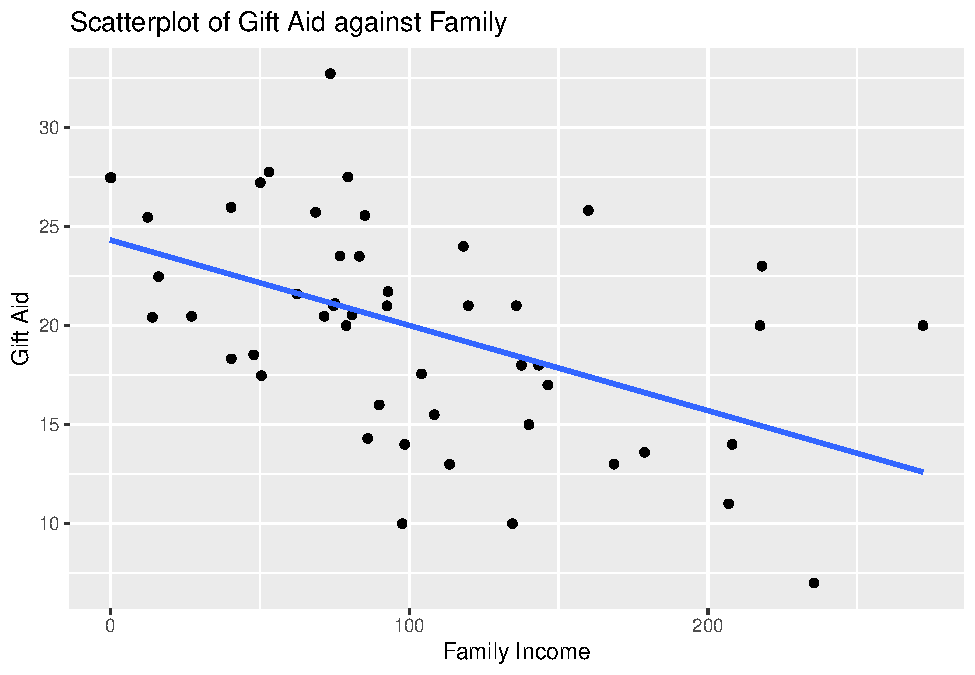
\includegraphics{bookdown-demo_files/figure-latex/unnamed-chunk-14-1.pdf}

We note that the observations are fairly evenly scattered on both sides of the regression line, so a linear association exists. We see a negative linear association. As family income increases, the gift aid, on average, decreases.

We also do not see any observation with weird values that may warrant further investigation.

\hypertarget{regression}{%
\subsection*{Regression}\label{regression}}
\addcontentsline{toc}{subsection}{Regression}

We use the \texttt{lm()} function to fit a regression model:

\begin{Shaded}
\begin{Highlighting}[]
\DocumentationTok{\#\#regress gift aid against family income}
\NormalTok{result}\OtherTok{\textless{}{-}}\FunctionTok{lm}\NormalTok{(gift\_aid}\SpecialCharTok{\textasciitilde{}}\NormalTok{family\_income, }\AttributeTok{data=}\NormalTok{Data)}
\end{Highlighting}
\end{Shaded}

Use the \texttt{summary()} function to display relevant information from this regression:

\begin{Shaded}
\begin{Highlighting}[]
\DocumentationTok{\#\#look at information regarding regression}
\FunctionTok{summary}\NormalTok{(result)}
\end{Highlighting}
\end{Shaded}

\begin{verbatim}
## 
## Call:
## lm(formula = gift_aid ~ family_income, data = Data)
## 
## Residuals:
##      Min       1Q   Median       3Q      Max 
## -10.1128  -3.6234  -0.2161   3.1587  11.5707 
## 
## Coefficients:
##               Estimate Std. Error t value Pr(>|t|)    
## (Intercept)   24.31933    1.29145  18.831  < 2e-16 ***
## family_income -0.04307    0.01081  -3.985 0.000229 ***
## ---
## Signif. codes:  0 '***' 0.001 '**' 0.01 '*' 0.05 '.' 0.1 ' ' 1
## 
## Residual standard error: 4.783 on 48 degrees of freedom
## Multiple R-squared:  0.2486, Adjusted R-squared:  0.2329 
## F-statistic: 15.88 on 1 and 48 DF,  p-value: 0.0002289
\end{verbatim}

We see the following values:

\begin{itemize}
\tightlist
\item
  \(\hat{\beta}_1 =\) -0.0430717. The estimated slope informs us the the predicted gift aid decreases by 0.0430717 thousands of dollars (or \$43.07) per unit increase in family income.
\item
  \(\hat{\beta}_0 =\) 24.319329. For students with no family income, their predicted gift aid is \$24 319.33. Note: from the scatterplot, we have an observation with 0 family income. We must be careful in not extrapolating when making predictions with our regression. We should only make predictions for family incomes between the minimum and maximum values of family incomes in our data.
\item
  \(s\) = 4.7825989, is the estimate of the standard deviation of the error terms. This is reported as residual standard error in R. Squaring this gives the estimated variance.
\item
  \(F\) = 15.8772043. This is the value of the ANOVA \(F\) statistic. The corresponding p-value is reported. Since this p-value is very small, we reject the null hypothesis. The data support the claim that there is a linear association between gift aid and family income.
\item
  \(R^2 =\) 0.2485582. The coefficient of determination informs us that about 24.86\% of the variation in gift aid can be explained by family income.
\end{itemize}

\hypertarget{extract-values-from-r-objects}{%
\subsubsection*{Extract values from R objects}\label{extract-values-from-r-objects}}
\addcontentsline{toc}{subsubsection}{Extract values from R objects}

We can actually extract these values that are being reported from \texttt{summary(result)}. To see what can be extracted from an R object, use the \texttt{names()} function:

\begin{Shaded}
\begin{Highlighting}[]
\DocumentationTok{\#\#see what can be extracted from summary(result)}
\FunctionTok{names}\NormalTok{(}\FunctionTok{summary}\NormalTok{(result))}
\end{Highlighting}
\end{Shaded}

\begin{verbatim}
##  [1] "call"          "terms"         "residuals"     "coefficients" 
##  [5] "aliased"       "sigma"         "df"            "r.squared"    
##  [9] "adj.r.squared" "fstatistic"    "cov.unscaled"
\end{verbatim}

To extract the estimated coefficients:

\begin{Shaded}
\begin{Highlighting}[]
\DocumentationTok{\#\#extract coefficients}
\FunctionTok{summary}\NormalTok{(result)}\SpecialCharTok{$}\NormalTok{coefficients}
\end{Highlighting}
\end{Shaded}

\begin{verbatim}
##                  Estimate Std. Error   t value     Pr(>|t|)
## (Intercept)   24.31932901 1.29145027 18.831022 8.281020e-24
## family_income -0.04307165 0.01080947 -3.984621 2.288734e-04
\end{verbatim}

Notice the information is presented in a table. To extract a specific value, we can specify the row and column indices:

\begin{Shaded}
\begin{Highlighting}[]
\DocumentationTok{\#\#extract slope}
\FunctionTok{summary}\NormalTok{(result)}\SpecialCharTok{$}\NormalTok{coefficients[}\DecValTok{2}\NormalTok{,}\DecValTok{1}\NormalTok{]}
\end{Highlighting}
\end{Shaded}

\begin{verbatim}
## [1] -0.04307165
\end{verbatim}

\begin{Shaded}
\begin{Highlighting}[]
\DocumentationTok{\#\#extract intercept}
\FunctionTok{summary}\NormalTok{(result)}\SpecialCharTok{$}\NormalTok{coefficients[}\DecValTok{1}\NormalTok{,}\DecValTok{1}\NormalTok{]}
\end{Highlighting}
\end{Shaded}

\begin{verbatim}
## [1] 24.31933
\end{verbatim}

On your own, extract the values of the residual standard error, the ANOVA F statistic, and \(R^2\).

\hypertarget{prediction}{%
\subsubsection*{Prediction}\label{prediction}}
\addcontentsline{toc}{subsubsection}{Prediction}

A use of regression models is prediction. Suppose I want to predict the gift aid of a student with family income of 50 thousand dollars (assuming the unit is in thousands of dollars). We use the \texttt{predict()} function:

\begin{Shaded}
\begin{Highlighting}[]
\DocumentationTok{\#\#create data point for prediction}
\NormalTok{newdata}\OtherTok{\textless{}{-}}\FunctionTok{data.frame}\NormalTok{(}\AttributeTok{family\_income=}\DecValTok{50}\NormalTok{)}
\DocumentationTok{\#\#predicted gift aid when x=50}
\FunctionTok{predict}\NormalTok{(result,newdata)}
\end{Highlighting}
\end{Shaded}

\begin{verbatim}
##        1 
## 22.16575
\end{verbatim}

This student's predicted gift aid is \$22 165.75. Alternatively, you could have calculated this by plugging \(x=50\) into the estimated SLR equation:

\begin{Shaded}
\begin{Highlighting}[]
\FunctionTok{summary}\NormalTok{(result)}\SpecialCharTok{$}\NormalTok{coefficients[}\DecValTok{1}\NormalTok{,}\DecValTok{1}\NormalTok{] }\SpecialCharTok{+} \FunctionTok{summary}\NormalTok{(result)}\SpecialCharTok{$}\NormalTok{coefficients[}\DecValTok{2}\NormalTok{,}\DecValTok{1}\NormalTok{]}\SpecialCharTok{*}\DecValTok{50}
\end{Highlighting}
\end{Shaded}

\begin{verbatim}
## [1] 22.16575
\end{verbatim}

\hypertarget{anova-table-1}{%
\subsubsection*{ANOVA table}\label{anova-table-1}}
\addcontentsline{toc}{subsubsection}{ANOVA table}

We use the \texttt{anova()} function to display the ANOVA table

\begin{Shaded}
\begin{Highlighting}[]
\NormalTok{anova.tab}\OtherTok{\textless{}{-}}\FunctionTok{anova}\NormalTok{(result)}
\NormalTok{anova.tab}
\end{Highlighting}
\end{Shaded}

\begin{verbatim}
## Analysis of Variance Table
## 
## Response: gift_aid
##               Df  Sum Sq Mean Sq F value    Pr(>F)    
## family_income  1  363.16  363.16  15.877 0.0002289 ***
## Residuals     48 1097.92   22.87                      
## ---
## Signif. codes:  0 '***' 0.001 '**' 0.01 '*' 0.05 '.' 0.1 ' ' 1
\end{verbatim}

The report \(F\) statistic is the same as the value reported earlier from \texttt{summary(result)}.

The first line of the output gives \(SS_{R}\), the second line gives \(SS_{res}\). The function doesn't provide \(SS_T\), but we know that \(SS_T = SS_{R} + SS_{res}\).

Again, to see what can be extracted from \texttt{anova.tab}:

\begin{Shaded}
\begin{Highlighting}[]
\FunctionTok{names}\NormalTok{(anova.tab)}
\end{Highlighting}
\end{Shaded}

\begin{verbatim}
## [1] "Df"      "Sum Sq"  "Mean Sq" "F value" "Pr(>F)"
\end{verbatim}

So \(SS_T\) can be easily calculated:

\begin{Shaded}
\begin{Highlighting}[]
\NormalTok{SST}\OtherTok{\textless{}{-}}\FunctionTok{sum}\NormalTok{(anova.tab}\SpecialCharTok{$}\StringTok{"Sum Sq"}\NormalTok{)}
\NormalTok{SST}
\end{Highlighting}
\end{Shaded}

\begin{verbatim}
## [1] 1461.079
\end{verbatim}

The \(R^2\) was reported to be 0.2485582. To verify using the ANOVA table:

\begin{Shaded}
\begin{Highlighting}[]
\NormalTok{anova.tab}\SpecialCharTok{$}\StringTok{"Sum Sq"}\NormalTok{[}\DecValTok{1}\NormalTok{]}\SpecialCharTok{/}\NormalTok{SST}
\end{Highlighting}
\end{Shaded}

\begin{verbatim}
## [1] 0.2485582
\end{verbatim}

\hypertarget{correlation-1}{%
\subsection*{Correlation}\label{correlation-1}}
\addcontentsline{toc}{subsection}{Correlation}

We use the \texttt{cor()} function to find the correlation between two quantitative variables:

\begin{Shaded}
\begin{Highlighting}[]
\DocumentationTok{\#\#correlation}
\FunctionTok{cor}\NormalTok{(Data}\SpecialCharTok{$}\NormalTok{family\_income,Data}\SpecialCharTok{$}\NormalTok{gift\_aid)}
\end{Highlighting}
\end{Shaded}

\begin{verbatim}
## [1] -0.4985561
\end{verbatim}

The correlation is -0.4985561. We have a moderate, negative linear association between family income and gift aid.

\hypertarget{inf}{%
\chapter{Inference with Simple Linear Regression (SLR)}\label{inf}}

\hypertarget{introduction}{%
\section{Introduction}\label{introduction}}

Oftentimes, the data we collect come from a random sample that is representative of the population of interest. A common example is an election poll before a presidential election. Random sampling allows the sample to be representative of the population. However, if we obtain another random sample, the characteristics of the new sample are unlikely to be exactly the same as the first sample. For example, the sample proportion who will vote for a certain party is unlikely to be the same for both random samples. What this tells us is that even with representative samples, sample proportions are unlikely to be equal to the population proportion, and sample proportions vary from sample to sample.

Dr.~W. Edwards Deming's Red Bead experiment illustrates this concept. A video of this experiment \href{https://www.youtube.com/watch?v=R3ewHrpqclA}{can be found here.}

In this video, the number of red beads, which represent bad products, varies each time the worker obtains a random sample of 50 beads. The fact that the number of red beads increases in his second sample does not indicate that he performed his task any worse, as this increase is due to the random variation associated with samples.

Note: Deming's Red Bead experiment was developed to illustrate concepts associated with management. He is best known for his work in developing the Japanese economy after World War II. You will be able to find many blogs/articles discussing the experiment on the World Wide Web. Although many of the articles discuss how this experiment applies in management, it can be used to illustrate concepts of variation.

The same idea extends to the slope and intercept of a regression line. The estimated slope and intercept will vary from sample to sample and are unlikely to be equal to the population slope and intercept. In inferential statistics, we use hypothesis tests and confidence intervals to aid us in accounting for this random variation. In this module, you will learn how to account for and quantify the random variation associated with the estimated regression model, and how to interpret the estimated regression model while accounting for random variation.

\hypertarget{review-from-previous-module}{%
\subsection{Review from previous module}\label{review-from-previous-module}}

The \textbf{simple linear regression model} is written as

\begin{equation}
y=\beta_0+\beta_{1} x + \epsilon. 
\label{eq:4SLRmod}
\end{equation}

We make some assumptions for the error term \(\epsilon\). They are:

\begin{enumerate}
\def\labelenumi{\arabic{enumi}.}
\tightlist
\item
  The errors have mean 0.
\item
  The \textbf{errors have variance denoted by \(\sigma^2\)}. Notice this variance is constant.
\item
  The errors are independent.
\item
  The errors are normally distributed.
\end{enumerate}

These assumptions allow us to derive the distributional properties associated with our least squares estimators \(\hat{\beta}_0, \hat{\beta}_1\), which then enables us to compute reliable confidence intervals and perform hypothesis tests on our SLR reliably.

\(\hat{\beta}_1,\hat{\beta}_0\) are the estimators for \(\beta_1,\beta_0\) respectively. These estimators can be interpreted in the following manner:

\begin{itemize}
\tightlist
\item
  \textbf{\(\hat{\beta}_1\) denotes the change in the predicted \(y\) when \(x\) increases by 1 unit. Alternatively, it denotes the change in \(y\), on average, when \(x\) increases by 1 unit.}
\item
  \textbf{\(\hat{\beta}_0\) denotes the predicted \(y\) when \(x=0\). Alternatively, it denotes the average of \(y\) when \(x=0\).}
\end{itemize}

How do the values of these estimators vary from sample to sample?

\hypertarget{hypothesis-testing-in-slr}{%
\section{Hypothesis Testing in SLR}\label{hypothesis-testing-in-slr}}

\hypertarget{distribution-of-least-squares-estimators}{%
\subsection{Distribution of least squares estimators}\label{distribution-of-least-squares-estimators}}

\textbf{Gauss Markov Theorem}: Under assumptions for a regression model, the least squares estimators \(\hat{\beta}_1\) and \(\hat{\beta}_0\) are unbiased and have minimum variance among all unbiased linear estimators.

Thus, the least squares estimators have the following properties:

\begin{enumerate}
\def\labelenumi{\arabic{enumi}.}
\tightlist
\item
  \(\mbox{E}(\hat{\beta}_1) = \beta_1\), \(\mbox{E}(\hat{\beta}_0) = \beta_0\)
\end{enumerate}

Note: An estimator is \textbf{unbiased} if its expected value is exactly equal to the parameter it is estimating.

\begin{enumerate}
\def\labelenumi{\arabic{enumi}.}
\setcounter{enumi}{1}
\tightlist
\item
  The variance of \(\hat{\beta}_1\) is
\end{enumerate}

\begin{equation} 
\mbox{Var}(\hat{\beta}_1) = \frac{\sigma^{2}}{\sum{(x_{i}-\bar{x})^{2}}}
\label{eq:4varb1}
\end{equation}

\begin{enumerate}
\def\labelenumi{\arabic{enumi}.}
\setcounter{enumi}{2}
\tightlist
\item
  The variance of \(\hat{\beta}_0\) is
\end{enumerate}

\begin{equation} 
\mbox{Var}(\hat{\beta}_0) = \sigma^2 \left[\frac{1}{n} + \frac{\bar{x}^2}{\sum (x_i -\bar{x})^2}\right]
\label{eq:4varb0}
\end{equation}

\begin{enumerate}
\def\labelenumi{\arabic{enumi}.}
\setcounter{enumi}{3}
\tightlist
\item
  \(\hat{\beta}_1\) and \(\hat{\beta}_0\) both follow a normal distribution.
\end{enumerate}

Note that in \eqref{eq:4varb1} and \eqref{eq:4varb0}, we use \(s^2 = MS_{res}\) to estimate \(\sigma^2\) since \(\sigma^2\) is a unknown value.

What these imply is that if we standardize \(\hat{\beta}_1\) and \(\hat{\beta}_0\), these standardized quantities will follow a \(t_{n-2}\) distribution, i.e.

\begin{equation} 
\frac{\hat{\beta}_1 - \beta_1}{se(\hat{\beta}_1)}\sim t_{n-2}
\label{eq:distb1}
\end{equation}

and

\begin{equation} 
\frac{\hat{\beta}_0 - \beta_0}{se(\hat{\beta}_0)}\sim t_{n-2},
\label{eq:distb0}
\end{equation}

where

\begin{equation}
se(\hat{\beta}_1) = \sqrt{\frac{MS_{res}}{\sum{(x_{i}-\bar{x})^{2}}}} = \frac{s}{\sqrt{\sum{(x_{i}-\bar{x})^{2}}}}
\label{eq:seb1}
\end{equation}

and

\begin{equation} 
se(\hat{\beta}_0) = \sqrt{MS_{res}\left[\frac{1}{n} + \frac{\bar{x}^2}{\sum (x_i -\bar{x})^2}\right]} = s \sqrt{\frac{1}{n} + \frac{\bar{x}^2}{\sum (x_i -\bar{x})^2}}
\label{eq:seb0}
\end{equation}

Note:

\begin{itemize}
\item
  \(se(\hat{\beta}_1)\) is read as the \textbf{standard error of \(\hat{\beta}_1\)}. The standard error of any estimator is essentially the sample standard deviation of that estimator, and measures the spread of that estimator.
\item
  A \(t_{n-2}\) distribution is read as a \textbf{\(t\) distribution with \(n-2\) degrees of freedom}.
\end{itemize}

\hypertarget{testing-regression-coefficients}{%
\subsection{Testing regression coefficients}\label{testing-regression-coefficients}}

Hypothesis testing is used to investigate if a population parameter is \textbf{different from a specific value}. In the context of SLR, we usually want to test if \(\beta_1\) is 0 or not. If \(\beta_1 = 0\), there is no linear relationship between the variables.

The general steps in hypothesis testing are:

\begin{itemize}
\tightlist
\item
  Step 1: State the null and alternative hypotheses.
\item
  Step 2: A test statistic is calculated using the sample, assuming the null is true. The value of the test statistic measures how the \textbf{sample deviates from the null}.
\item
  Step 3: Make conclusion, using either critical values or p-values.
\end{itemize}

In the previous module, we introduced the ANOVA \(F\) test. In SLR, this tests if the slope of the SLR equation is 0 or not. It turns out that we can also perform a \(t\) test for the slope. In the \(t\) test for the slope, the null and alternative hypotheses are:

\[
H_0: \beta_1 = 0, H_a: \beta_1 \neq 0.
\]
The test statistic is

\begin{equation} 
t = \frac{\hat{\beta}_1 - \text{ value in null}}{se(\hat{\beta}_1)}
\label{eq:4ttest}
\end{equation}

which is compared with a \(t_{n-2}\) distribution. Notice that \eqref{eq:4ttest} comes from \eqref{eq:distb1}.

Let us go back to our simulated example that we saw in the last module. We have data from 6000 UVa undergraduate students on the amount of time they spend studying in a week (in minutes), and how many courses they are taking in the semester (3 or 4 credit courses).

\begin{Shaded}
\begin{Highlighting}[]
\DocumentationTok{\#\#create dataframe}
\NormalTok{df}\OtherTok{\textless{}{-}}\FunctionTok{data.frame}\NormalTok{(study,courses)}

\DocumentationTok{\#\#fit regression}
\NormalTok{result}\OtherTok{\textless{}{-}}\FunctionTok{lm}\NormalTok{(study}\SpecialCharTok{\textasciitilde{}}\NormalTok{courses, }\AttributeTok{data=}\NormalTok{df)}
\DocumentationTok{\#\#look at regression coefficients}
\FunctionTok{summary}\NormalTok{(result)}\SpecialCharTok{$}\NormalTok{coefficients}
\end{Highlighting}
\end{Shaded}

\begin{verbatim}
##              Estimate Std. Error   t value      Pr(>|t|)
## (Intercept)  58.44829  1.9218752  30.41211 4.652442e-189
## courses     120.39310  0.4707614 255.74125  0.000000e+00
\end{verbatim}

The \(t\) statistic for testing \(H_0: \beta_1 = 0, H_a: \beta_1 \neq 0\) is reported to be 255.7412482, which can be calculated using \eqref{eq:4ttest}: \(t= \frac{120.39310 - 0}{0.4707614}\). The reported p-value is virtually 0, so we reject the null hypothesis. The data support the claim that there is a linear association between study time and the number of courses taken.

\hypertarget{confidence-intervals-for-regression-coefficients}{%
\section{Confidence Intervals for Regression Coefficients}\label{confidence-intervals-for-regression-coefficients}}

Confidence intervals (CIs) are similar to hypothesis testing in the sense that they are also based on the distributional properties of an estimator. CIs may differ in their use in the following ways:

\begin{enumerate}
\def\labelenumi{\arabic{enumi}.}
\tightlist
\item
  We are not assessing if the parameter is different from a specific value.
\item
  We are more interested in exploring a plausible \textbf{range of values for an unknown parameter}.
\end{enumerate}

Because CIs and hypothesis tests are based on the distributional properties of an estimator, their conclusions will be consistent (as long as the significance level is the same).

Recall the general form for CIs:

\begin{equation} 
\mbox{estimator} \pm (\mbox{multiplier} \times \mbox{s.e of estimator}). 
\label{eq:4CI}
\end{equation}

We have the following components of a CI

\begin{itemize}
\tightlist
\item
  \textbf{estimator (or statistic)}: numerical quantity that describes a sample
\item
  \textbf{multiplier}: determined by confidence level and relevant probability distribution
\item
  \textbf{standard error of estimator}: measure of variance of estimator (basically the square root of the variance of estimator)
\end{itemize}

Following \eqref{eq:4CI} and \eqref{eq:distb1}, the \(100(1-\alpha)\%\) CI for \(\beta_1\) is

\begin{equation} 
\hat{\beta}_1 \pm t_{1-\alpha/2;n-2}  se(\hat{\beta}_1) = \hat{\beta}_1 \pm t_{1-\alpha/2;n-2} \frac{s}{\sqrt{\sum(x_i - \bar{x})^{2}}}.
\label{eq:4CIb1}
\end{equation}

Going back to our study time example, the 95\% CI for \(\beta_1\) is (119.470237, 121.3159601).

\begin{Shaded}
\begin{Highlighting}[]
\DocumentationTok{\#\#CI for coefficients}
\FunctionTok{confint}\NormalTok{(result,}\AttributeTok{level =} \FloatTok{0.95}\NormalTok{)[}\DecValTok{2}\NormalTok{,]}
\end{Highlighting}
\end{Shaded}

\begin{verbatim}
##    2.5 %   97.5 % 
## 119.4702 121.3160
\end{verbatim}

An interpretation of this CI is that we have 95\% confidence that the true slope \(\beta_1\) lies between (119.470237, 121.3159601). In other words, for each additional course taken, the predicted study time increases between 119.470237 and 121.3159601 minutes.

\hypertarget{thought-questions}{%
\subsection{Thought questions}\label{thought-questions}}

\begin{itemize}
\item
  Is the conclusion from this 95\% CI consistent with the hypothesis test for \(H_0: \beta_1 = 0\) in the previous section at 0.05 significance level?
\item
  I have presented hypothesis tests and CIs for the slope, \(\beta_1\).

  \begin{itemize}
  \item
    How would you calculate the \(t\) statistic if you wanted to test \(H_0: \beta_0 = 0, H_0: \beta_0 \neq 0\)?
  \item
    How would you calculate the 95\% CI for the intercept \(\beta_0\)?
  \end{itemize}
\end{itemize}

Generally, we are usually more interested in the slope than the intercept.

\hypertarget{ci-of-the-mean-response}{%
\section{CI of the Mean Response}\label{ci-of-the-mean-response}}

We have established that the least squares estimators \(\hat{\beta}_1,\hat{\beta}_0\) have their associated variances. Since the estimated SLR equation is

\begin{equation} 
\hat{y}=\hat{\beta}_0+\hat{\beta}_1 x,
\label{eq:4fitted}
\end{equation}

it stands to reason that \(\hat{y}\) has an associated variance as well, since it is a function of \(\hat{\beta}_1,\hat{\beta}_0\).

There are two interpretations of \(\hat{y}\):

\begin{enumerate}
\def\labelenumi{\arabic{enumi}.}
\tightlist
\item
  it \textbf{estimates the mean of \(y\) when \(x=x_0\)};
\item
  it \textbf{predicts the value of \(y\) for a new observation when \(x=x_0\)}.
\end{enumerate}

Note: \(x_0\) denotes a specific numerical value for the predictor variable.

Depending on which interpretation we want, there are two different intervals based on \(\hat{y}\). The first interpretation is associated with the \textbf{confidence interval for the mean response, \(\hat{\mu}_{y|x_0}\), given the predictor}. This is used when we are interested in the average value of the response variable, when the predictor is equal to a specific value. This CI is

\begin{equation} 
\hat{\mu}_{y|x_0}\pm t_{1-\alpha/2,n-2}s\sqrt{\frac{1}{n} +
\frac{(x_0-\bar{x})^2}{\sum(x_i-\bar{x})^2}}.
\label{eq:4CImean}
\end{equation}

Going back to our study time example, suppose we want the average study time for students who take 5 courses, the 95\% CI is

\begin{Shaded}
\begin{Highlighting}[]
\DocumentationTok{\#\#CI for mean y when x=5}
\NormalTok{newdata}\OtherTok{\textless{}{-}}\FunctionTok{data.frame}\NormalTok{(}\AttributeTok{courses=}\DecValTok{5}\NormalTok{)}
\FunctionTok{predict}\NormalTok{(result, newdata, }\AttributeTok{level=}\FloatTok{0.95}\NormalTok{, }\AttributeTok{interval=}\StringTok{"confidence"}\NormalTok{)}
\end{Highlighting}
\end{Shaded}

\begin{verbatim}
##        fit      lwr      upr
## 1 660.4138 659.2224 661.6052
\end{verbatim}

We have 95\% confidence that the average study time for students who take 5 courses is between 659.2223688 and 661.605187 minutes.

\hypertarget{pi-of-a-new-response}{%
\section{PI of a New Response}\label{pi-of-a-new-response}}

Previously, we found a CI for the mean of \(y\) given a specific value of \(x\), \eqref{eq:4CImean}. This CI gives us an idea about the location of the regression line at a specific of \(x\).

Instead, we may have interest in finding an interval for a new value of \(\hat{y}_0\), when we have a new observation \(x=x_0\). This is called a \textbf{prediction interval (PI) for a future observation \(y_0\) when the predictor is a specific value}. This interval follows from the second interpretation of \(\hat{y}\).

The PI for \(\hat{y}_0\) takes into account:

\begin{enumerate}
\def\labelenumi{\arabic{enumi}.}
\tightlist
\item
  Variation in location for the distribution of \(y\) (i.e.~where is the center of the distribution of \(y\)?).
\item
  Variation \textbf{within the probability distribution of \(y\)}.
\end{enumerate}

By comparison, the confidence interval for the mean response \eqref{eq:4CImean} only takes into account the first element. The PI is

\begin{equation} 
\hat{y}_0\pm t_{1-\alpha/2,n-2}s \sqrt{1+\frac{1}{n} +
\frac{(x_0-\bar{x})^2}{\sum(x_i-\bar{x})^2}}.
\label{eq:4pred}
\end{equation}

Going back to our study time example, suppose we have a newly enrolled student who wishes to take 5 courses, and the student wants to predict his study time

\begin{Shaded}
\begin{Highlighting}[]
\DocumentationTok{\#\#PI for y when x=5}
\FunctionTok{predict}\NormalTok{(result, newdata, }\AttributeTok{level=}\FloatTok{0.95}\NormalTok{, }\AttributeTok{interval=}\StringTok{"prediction"}\NormalTok{)}
\end{Highlighting}
\end{Shaded}

\begin{verbatim}
##        fit      lwr      upr
## 1 660.4138 602.0347 718.7928
\end{verbatim}

We have 95\% confidence that the study time for this student is between 602.0347305 and 718.7928253 minutes.

\hypertarget{thought-questions-1}{%
\subsection{Thought questions}\label{thought-questions-1}}

\begin{itemize}
\item
  In the following two scenarios, decide if we are more interested in the CI for the mean response given the predictor \eqref{eq:4CImean}, or the PI for a future response given the predictor \eqref{eq:4pred}.

  \begin{itemize}
  \item
    We wish to estimate the waiting time, on average, of DMV customers if there are 10 people in line at the DMV.
  \item
    I enter the DMV and notice 10 people in line. I want to estimate my waiting time.
  \end{itemize}
\item
  Look at the standard errors associated with the intervals given in \eqref{eq:4CImean} and \eqref{eq:4pred}. How are they related to each other?
\end{itemize}

\hypertarget{supplemental-notes-on-statistical-inference}{%
\section{Supplemental Notes on Statistical Inference}\label{supplemental-notes-on-statistical-inference}}

\hypertarget{hypothesis-statements}{%
\subsection{Hypothesis statements}\label{hypothesis-statements}}

Let's consider a \(t\) test for the regression parameter, \(\beta_1\). Depending on context, the following could be null and alternative hypotheses

\begin{itemize}
\tightlist
\item
  \(H_0: \beta_1 = 0, H_a: \beta_1 \neq 0\).
\item
  \(H_0: \beta_1 = 0, H_a: \beta_1 > 0\).
\item
  \(H_0: \beta_1 = 0, H_a: \beta_1 < 0\).
\end{itemize}

The null hypothesis should be stated as a statement of \textbf{equality}. This concept holds true for hypothesis tests in general. Some other books / resources might state them as

\begin{itemize}
\tightlist
\item
  \(H_0: \beta_1 = 0, H_a: \beta_1 \neq 0\).
\item
  \(H_0: \beta_1 \leq 0, H_a: \beta_1 > 0\).
\item
  \(H_0: \beta_1 \geq 0, H_a: \beta_1 < 0\).
\end{itemize}

I prefer using the equality statement for the null hypothesis for the following reasons (theoretical, pedagogical, practical):

\begin{enumerate}
\def\labelenumi{\arabic{enumi}.}
\tightlist
\item
  The null hypothesis being an equality aligns with the definition of the p-value.
\end{enumerate}

\begin{itemize}
\tightlist
\item
  The p-value is the probability of observing our sample estimate (or a value more extreme), if the null hypothesis is true (i.e.~\(\beta_1\) is truly 0). This is what we are assuming in the calculation for the test statistic.
\end{itemize}

\begin{enumerate}
\def\labelenumi{\arabic{enumi}.}
\setcounter{enumi}{1}
\tightlist
\item
  People tend to get confused between the null and alternative hypotheses if both involve inequalities (the alternative is the hypothesis you are trying to support).
\item
  Conclusions are made in terms of supporting (or not supporting) the alternative hypothesis.
\end{enumerate}

\hypertarget{sample-size-and-statistical-inference}{%
\subsection{Sample size and statistical inference}\label{sample-size-and-statistical-inference}}

Generally speaking, there is a relationship between sample size and statistical inference (assuming other characteristics remain the same and our sample was randomly obtained or representative of the population of interest):

\begin{itemize}
\tightlist
\item
  Larger sample sizes (typically) lead to narrower confidence intervals (more precise intervals).
\item
  Sample estimates based on larger samples are more likely to be closer to the true parameters.
\item
  Larger sample (typically) lead to more evidence against the null hypothesis.

  \begin{itemize}
  \tightlist
  \item
    This means a larger sample size leads to a more powerful test. The power of a test is the probability a hypothesis test is able to correctly reject the null hypothesis.
  \end{itemize}
\end{itemize}

\hypertarget{small-sample-sizes}{%
\subsubsection{Small sample sizes}\label{small-sample-sizes}}

Small sample sizes tend to result in:

\begin{itemize}
\tightlist
\item
  Confidence intervals that are wide.
\item
  Sample estimates that are more likely to be further away from the true parameters.
\item
  Hypothesis tests that are more likely to incorrectly fail to reject the null hypothesis when the alternative hypothesis is true.
\end{itemize}

While larger sample sizes have their advantages, there are also some disadvantages with sample sizes that are extremely large.

\hypertarget{large-sample-sizes}{%
\subsubsection{Large sample sizes}\label{large-sample-sizes}}

A ``statistically significant'' result does not necessarily mean that the result has practical consequences. Suppose a 95\% confidence interval for \(\beta_1\) is \((0.001, 0.002)\). The interval excludes 0, so it is ``statistically significantly'' different from 0 (because it is!), but does this result have practical consequences? A narrow CI that barely excludes the null value can happen when we have a large sample size.

If one was to conduct the corresponding hypothesis test, we would reject the null hypothesis that \(\beta_1 = 0\). With large sample sizes, hypothesis tests are sensitive to small departures from the null hypothesis.

In such instances, it may be worth considering hypothesis tests involving a different value in the null hypothesis, one that makes sense for your question. For example, a practically significant slope may need to be greater than a specific numerical value for a certain context.

\begin{itemize}
\tightlist
\item
  Statistical inference to assess statistical significance.
\item
  Subject area knowledge to assess practical significance.
\end{itemize}

\hypertarget{questions}{%
\subsubsection{Questions}\label{questions}}

Are the following results statistically significant? If so, are the results also practically significant? Assume a two-sided test with a null value of 0 (These are made up examples):

\begin{enumerate}
\def\labelenumi{\arabic{enumi}.}
\item
  In assessing if studying more is associated with better test scores, a SLR is carried out with test scores (out of 100 points) against study time (in hours). The 95\% confidence interval for the slope \(\beta_1\) is (5.632, 7.829).
\item
  A SLR is carried out to explore the linear relationship between number of years in school with income (in thousands of dollars). The 95\% confidence interval for the slope \(\beta_1\) is (0.051, 0.243).
\end{enumerate}

\hypertarget{cautions-using-slr-and-correlation}{%
\subsection{Cautions using SLR and Correlation}\label{cautions-using-slr-and-correlation}}

Simple linear regression and correlation are meant for assessing \textbf{linear} relationships. If the relationship is not linear, we will need to transform the variable(s) (so the transformed variables have a linear relationship. Will explore this in Module \ref{diag}).

\begin{itemize}
\tightlist
\item
  Always verify via a scatterplot that the relationship is at least approximately linear.
\item
  A high correlation or a significant estimated slope by themselves do not prove that we have a strong linear relationship between the variables. Conversely, a correlation close to 0 or an insignificant estimated slope is also not proof that we do not have a relationship between the variables.
\end{itemize}

\hypertarget{outliers}{%
\subsubsection{Outliers}\label{outliers}}

SLR and correlation are sensitive to outliers / influential observations. Generally speaking, these are data that are ``far away'' or very different from the rest of the observations. These data points can be visually inspected from a scatterplot. Some potential considerations when dealing with such data points:

\begin{itemize}
\tightlist
\item
  Investigate these observations. There is usually something that is making them ``stand out'' from the rest of the data.
\item
  Data entry errors that can be corrected. Be sure to mention in the report.
\item
  Revisit how the data were sampled. Perhaps the data point is is not part of the population of interest. If so, data point can be removed (this is legitimate), but be sure to mention in the report.
\end{itemize}

With regards to regression analysis:

\begin{itemize}
\tightlist
\item
  Exclusion of data points must be clearly documented.
\item
  Fit the regression with and without the data points in question, and see how similar or different the conclusions become.
\item
  If the data points have large value(s) on the predictor and/or response, a log transformation on the variable can pull in the large values.
\item
  Consider subsetting your data and create separate models for each subset; or focus on a subset and make it clear your analysis is for a subset.
\item
  Knowing your data and context can help a lot in these decisions.
\end{itemize}

\hypertarget{association-and-causation}{%
\subsubsection{Association and causation}\label{association-and-causation}}

Two correlated variables do not mean that one variable causes the other variable to change. For example, consider a plot of ice cream consumption and deaths by drowning during various months. There may be some positive correlation, and clearly, eating more ice cream does not cause more drownings. The correlation can be explained by a third (lurking) variable: the weather.

A \textbf{lurking variable} is a variable that has an impact on the relationship between the variables being studied, but is itself not studied.

A carefully designed \textbf{randomized experiment} can control for lurking variables, and causal relationships can be established. Typically, such experiments include:

\begin{itemize}
\tightlist
\item
  A control group and a treatment group.
\item
  Random assignment of large number of observations into the treatment and control groups. Due to the random assignment, the general characteristics of of subjects in each group are similar.
\end{itemize}

Lurking variables are always an issue with \textbf{observational studies}. Researchers in observational studies do not intervene with the observations and simply observe the data that the observations generate. Causal relationships are much more difficult to establish with observational studies.

\hypertarget{questions-1}{%
\subsubsection{Questions}\label{questions-1}}

\begin{enumerate}
\def\labelenumi{\arabic{enumi}.}
\item
  Consider the \texttt{palmerpenguins} dataset that we have been working on. The data contain size measurements for three different species of penguins on three islands in the Palmer Archipelago, Antarctica over three years. Is this an observational study or randomized experiment?
\item
  A fertilizer company wishes to evaluate how effective a new fertilizer is in terms of improving the yield of crops. A large field is divided into many smaller plots, and each smaller plot is randomly assigned to receive either the new fertilizer or the standard fertilizer. Is this an observational study or randomized experiment?
\item
  A professor wishes to evaluate the effectiveness of various teaching methods (traditional vs flipped classroom). The professor uses the traditional approach for a section that meets on Mondays, Wednesdays, and Fridays from 9 to 10am and uses the flipped classroom approach for a section that meets on Mondays, Wednesdays, and Fridays from 2 to 3pm. Students were free to choose whichever section that wanted to register for, with no knowledge of the teaching method being used. What are some potential lurking variables in this study?
\end{enumerate}

\hypertarget{r-tutorial-1}{%
\section{R Tutorial}\label{r-tutorial-1}}

For this tutorial, we will continue to work with the dataset \texttt{elmhurst} from the \texttt{openintro} package in R.

\begin{Shaded}
\begin{Highlighting}[]
\FunctionTok{library}\NormalTok{(tidyverse)}
\FunctionTok{library}\NormalTok{(openintro)}
\NormalTok{Data}\OtherTok{\textless{}{-}}\NormalTok{openintro}\SpecialCharTok{::}\NormalTok{elmhurst}
\end{Highlighting}
\end{Shaded}

The key pieces of information are:

\begin{itemize}
\tightlist
\item
  A random sample of 50 students (all freshman from the 2011 class at Elmhurst College).
\item
  Family income of the student (units are missing).
\item
  Gift aid, in \$1000s.
\end{itemize}

We want to explore how family income may be related to gift aid, in a simple linear regression framework.

\hypertarget{hypothesis-test-for-beta_1-and-beta_0}{%
\subsection*{\texorpdfstring{Hypothesis test for \(\beta_1\) (and \(\beta_0\))}{Hypothesis test for \textbackslash beta\_1 (and \textbackslash beta\_0)}}\label{hypothesis-test-for-beta_1-and-beta_0}}
\addcontentsline{toc}{subsection}{Hypothesis test for \(\beta_1\) (and \(\beta_0\))}

Applying the \texttt{summary()} function to \texttt{lm()} gives the results of hypothesis tests for \(\beta_1\) and \(\beta_0\):

\begin{Shaded}
\begin{Highlighting}[]
\DocumentationTok{\#\#Fit a regression model}
\NormalTok{result}\OtherTok{\textless{}{-}}\FunctionTok{lm}\NormalTok{(gift\_aid}\SpecialCharTok{\textasciitilde{}}\NormalTok{family\_income, }\AttributeTok{data=}\NormalTok{Data)}

\DocumentationTok{\#\#look at t stats and F stat}
\FunctionTok{summary}\NormalTok{(result)}
\end{Highlighting}
\end{Shaded}

\begin{verbatim}
## 
## Call:
## lm(formula = gift_aid ~ family_income, data = Data)
## 
## Residuals:
##      Min       1Q   Median       3Q      Max 
## -10.1128  -3.6234  -0.2161   3.1587  11.5707 
## 
## Coefficients:
##               Estimate Std. Error t value Pr(>|t|)    
## (Intercept)   24.31933    1.29145  18.831  < 2e-16 ***
## family_income -0.04307    0.01081  -3.985 0.000229 ***
## ---
## Signif. codes:  0 '***' 0.001 '**' 0.01 '*' 0.05 '.' 0.1 ' ' 1
## 
## Residual standard error: 4.783 on 48 degrees of freedom
## Multiple R-squared:  0.2486, Adjusted R-squared:  0.2329 
## F-statistic: 15.88 on 1 and 48 DF,  p-value: 0.0002289
\end{verbatim}

Under coefficients, we can see the results of the hypothesis tests for \(\beta_1\) and \(\beta_0\). Specifically, for \(\beta_1\):

\begin{itemize}
\tightlist
\item
  \(\hat{\beta}_1\) = -0.0430717
\item
  \(se(\hat{\beta}_1)\) = 0.0108095
\item
  the test statistic is \(t\) = -3.984621
\item
  the corresponding p-value is \ensuremath{2.2887345\times 10^{-4}}
\end{itemize}

You can work out the p-value using R (slight difference due to rounding):

\begin{Shaded}
\begin{Highlighting}[]
\DocumentationTok{\#\#pvalue}
\DecValTok{2}\SpecialCharTok{*}\FunctionTok{pt}\NormalTok{(}\SpecialCharTok{{-}}\FunctionTok{abs}\NormalTok{(}\SpecialCharTok{{-}}\FloatTok{3.985}\NormalTok{), }\AttributeTok{df =} \DecValTok{50{-}2}\NormalTok{)}
\end{Highlighting}
\end{Shaded}

\begin{verbatim}
## [1] 0.0002285996
\end{verbatim}

Or find the critical value using R:

\begin{Shaded}
\begin{Highlighting}[]
\DocumentationTok{\#\#critical value}
\FunctionTok{qt}\NormalTok{(}\DecValTok{1}\FloatTok{{-}0.05}\SpecialCharTok{/}\DecValTok{2}\NormalTok{, }\AttributeTok{df =} \DecValTok{50{-}2}\NormalTok{)}
\end{Highlighting}
\end{Shaded}

\begin{verbatim}
## [1] 2.010635
\end{verbatim}

Either way, we end up rejecting the null hypothesis. The data support the claim that there is a linear association between gift aid and family income.

Note:

\begin{itemize}
\item
  the \(t\) tests for regression coefficients are based on \(H_0: \beta_j = 0, H_a: \beta_j \neq 0\). The reported p-value is based on this set of null and alternative hypotheses. If your null and alternative hypotheses are different, you will need to compute your own test statistic and p-value.
\item
  For SLR, the two-sided \(t\) test for \(\beta_1\) gives the exact same result as the ANOVA \(F\) test. Notice the p-values are the same. The \(F\) statistic of \(15.88\) is the squared of the \(t\) statistic, \((-3.985)^2\).
\end{itemize}

\hypertarget{confidence-interval-for-beta_1-and-beta_0}{%
\subsection*{\texorpdfstring{Confidence interval for \(\beta_1\) (and \(\beta_0\))}{Confidence interval for \textbackslash beta\_1 (and \textbackslash beta\_0)}}\label{confidence-interval-for-beta_1-and-beta_0}}
\addcontentsline{toc}{subsection}{Confidence interval for \(\beta_1\) (and \(\beta_0\))}

To find the 95\% confidence intervals for the coefficients, we use the \texttt{confint()} function:

\begin{Shaded}
\begin{Highlighting}[]
\DocumentationTok{\#\#to produce 95\% CIs for all regression coefficients}
\FunctionTok{confint}\NormalTok{(result,}\AttributeTok{level =} \FloatTok{0.95}\NormalTok{)}
\end{Highlighting}
\end{Shaded}

\begin{verbatim}
##                     2.5 %      97.5 %
## (Intercept)   21.72269421 26.91596380
## family_income -0.06480555 -0.02133775
\end{verbatim}

The 95\% CI for \(\beta_1\) is (-0.0648056, -0.0213378). We have 95\% confidence that for each additional thousand dollars in family income, the predicted gift aid decreases between \$21.3378 and \$64.8056.

\hypertarget{confidence-interval-for-mean-response-for-given-x}{%
\subsection*{Confidence interval for mean response for given x}\label{confidence-interval-for-mean-response-for-given-x}}
\addcontentsline{toc}{subsection}{Confidence interval for mean response for given x}

Suppose we want a confidence interval for the average gift aid for Elmhurst College students with family income of 80 thousand dollars. We can use the \texttt{predict()} function:

\begin{Shaded}
\begin{Highlighting}[]
\DocumentationTok{\#\#to produce 95\% CI for the mean response when x=80, }
\NormalTok{newdata}\OtherTok{\textless{}{-}}\FunctionTok{data.frame}\NormalTok{(}\AttributeTok{family\_income=}\DecValTok{80}\NormalTok{)}
\FunctionTok{predict}\NormalTok{(result,newdata,}\AttributeTok{level=}\FloatTok{0.95}\NormalTok{, }\AttributeTok{interval=}\StringTok{"confidence"}\NormalTok{)}
\end{Highlighting}
\end{Shaded}

\begin{verbatim}
##       fit      lwr      upr
## 1 20.8736 19.43366 22.31353
\end{verbatim}

The 95\% CI for the mean gift aid for students with family income of 80 thousand dollars is (19.4336609, 22.3135327). We have 95\% confidence the mean gift aid for students with family income of 80 thousand dollars is between \$19 433.66 and \$22 313.53.

\hypertarget{prediction-interval-for-a-response-for-a-given-x}{%
\subsection*{Prediction interval for a response for a given x}\label{prediction-interval-for-a-response-for-a-given-x}}
\addcontentsline{toc}{subsection}{Prediction interval for a response for a given x}

For a prediction interval for the gift aid of an Elmhurst College student with family income of 80 thousand dollars:

\begin{Shaded}
\begin{Highlighting}[]
\DocumentationTok{\#\#and the 95\% PI for the response of an observation when x=80}
\FunctionTok{predict}\NormalTok{(result,newdata,}\AttributeTok{level=}\FloatTok{0.95}\NormalTok{, }\AttributeTok{interval=}\StringTok{"prediction"}\NormalTok{)}
\end{Highlighting}
\end{Shaded}

\begin{verbatim}
##       fit      lwr      upr
## 1 20.8736 11.15032 30.59687
\end{verbatim}

We have 95\% confidence that for an Elmhurst College student with family income of 80, this student's gift aid is between \$11 150.32 and \$30 596.87.

\hypertarget{visualization-of-ci-for-mean-response-given-x-and-pi-of-response-given-x}{%
\subsection*{Visualization of CI for mean response given x and PI of response given x}\label{visualization-of-ci-for-mean-response-given-x-and-pi-of-response-given-x}}
\addcontentsline{toc}{subsection}{Visualization of CI for mean response given x and PI of response given x}

When using the \texttt{ggplot()} function to create a scatterplot, we can overlay the SLR equation by adding a layer via \texttt{geom\_smooth(method\ =\ lm)}. By default, the CI for the mean response for each value of the predictor gets overlaid as well. In the previous tutorial, we removed this by adding \texttt{se=FALSE} inside \texttt{geom\_smooth()}:

\begin{Shaded}
\begin{Highlighting}[]
\DocumentationTok{\#\#regular scatterplot}
\DocumentationTok{\#\#with regression line overlaid, and bounds of CI for mean y}
\NormalTok{ggplot2}\SpecialCharTok{::}\FunctionTok{ggplot}\NormalTok{(Data, }\FunctionTok{aes}\NormalTok{(}\AttributeTok{x=}\NormalTok{family\_income, }\AttributeTok{y=}\NormalTok{gift\_aid))}\SpecialCharTok{+}
  \FunctionTok{geom\_point}\NormalTok{() }\SpecialCharTok{+}
  \FunctionTok{geom\_smooth}\NormalTok{(}\AttributeTok{method=}\NormalTok{lm)}\SpecialCharTok{+}
  \FunctionTok{labs}\NormalTok{(}\AttributeTok{x=}\StringTok{"Family Income"}\NormalTok{, }
       \AttributeTok{y=}\StringTok{"Gift Aid"}\NormalTok{, }
       \AttributeTok{title=}\StringTok{"Scatterplot of Gift Aid against Family Income"}\NormalTok{)}
\end{Highlighting}
\end{Shaded}

\begin{verbatim}
## `geom_smooth()` using formula = 'y ~ x'
\end{verbatim}

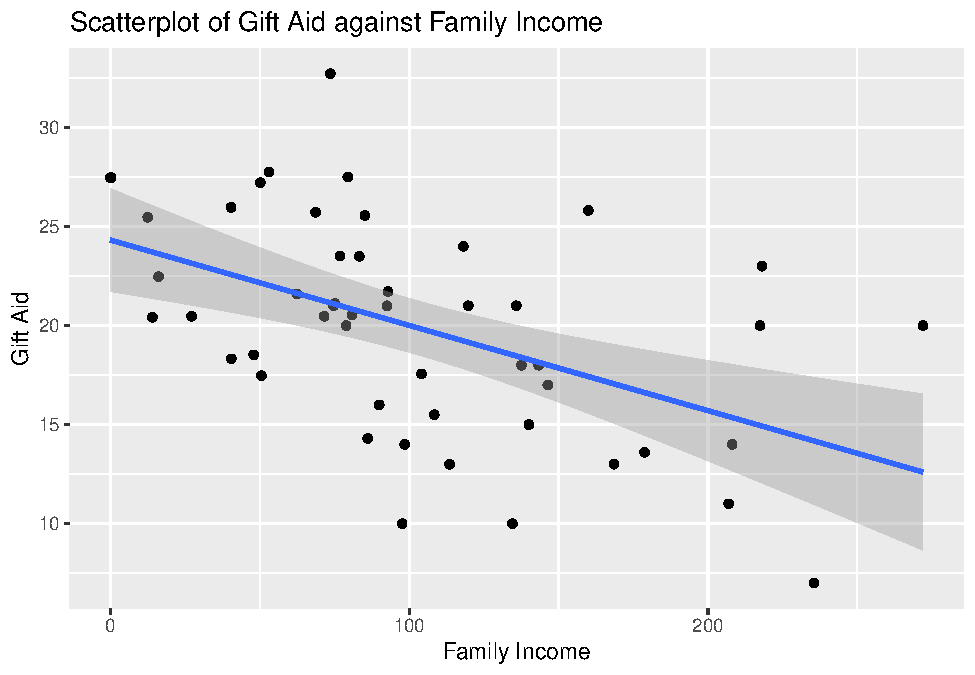
\includegraphics{bookdown-demo_files/figure-latex/unnamed-chunk-41-1.pdf}

Overlaying prediction intervals require a bit more work. We need to compute the lower and upper bounds of the PI for each value of the predictor:

\begin{Shaded}
\begin{Highlighting}[]
\DocumentationTok{\#\#find PIs for each observation}
\NormalTok{preds }\OtherTok{\textless{}{-}} \FunctionTok{predict}\NormalTok{(result, }\AttributeTok{interval=}\StringTok{"prediction"}\NormalTok{)}
\end{Highlighting}
\end{Shaded}

\begin{verbatim}
## Warning in predict.lm(result, interval = "prediction"): predictions on current data refer to _future_ responses
\end{verbatim}

Previously, when we used the \texttt{predict()} function, we provided the numerical value of \(x\) to make a prediction on. If this is not supplied, the function will use all the current values of \(x\) to make predictions, and will actually print out a warning message. For our purpose, this is not an issue since this is exactly what we want.

We then add \texttt{preds} to the data frame in order to overlay the lower and upper bounds on the scatterplot, by adding extra layers via \texttt{geom\_line()} in the \texttt{ggplot()} function:

\begin{Shaded}
\begin{Highlighting}[]
\DocumentationTok{\#\#add preds to data frame}
\NormalTok{Data}\OtherTok{\textless{}{-}}\FunctionTok{data.frame}\NormalTok{(Data,preds)}

\DocumentationTok{\#\#overlay PIs via geom\_line()}
\NormalTok{ggplot2}\SpecialCharTok{::}\FunctionTok{ggplot}\NormalTok{(Data, }\FunctionTok{aes}\NormalTok{(}\AttributeTok{x=}\NormalTok{family\_income, }\AttributeTok{y=}\NormalTok{gift\_aid))}\SpecialCharTok{+}
  \FunctionTok{geom\_point}\NormalTok{() }\SpecialCharTok{+}
  \FunctionTok{geom\_line}\NormalTok{(}\FunctionTok{aes}\NormalTok{(}\AttributeTok{y=}\NormalTok{lwr), }\AttributeTok{color =} \StringTok{"red"}\NormalTok{, }\AttributeTok{linetype =} \StringTok{"dashed"}\NormalTok{)}\SpecialCharTok{+}
  \FunctionTok{geom\_line}\NormalTok{(}\FunctionTok{aes}\NormalTok{(}\AttributeTok{y=}\NormalTok{upr), }\AttributeTok{color =} \StringTok{"red"}\NormalTok{, }\AttributeTok{linetype =} \StringTok{"dashed"}\NormalTok{)}\SpecialCharTok{+}
  \FunctionTok{geom\_smooth}\NormalTok{(}\AttributeTok{method=}\NormalTok{lm)}\SpecialCharTok{+}
  \FunctionTok{labs}\NormalTok{(}\AttributeTok{x=}\StringTok{"Family Income"}\NormalTok{, }
       \AttributeTok{y=}\StringTok{"Gift Aid"}\NormalTok{, }
       \AttributeTok{title=}\StringTok{"Scatterplot of Gift Aid against Family Income"}\NormalTok{)}
\end{Highlighting}
\end{Shaded}

\begin{verbatim}
## `geom_smooth()` using formula = 'y ~ x'
\end{verbatim}

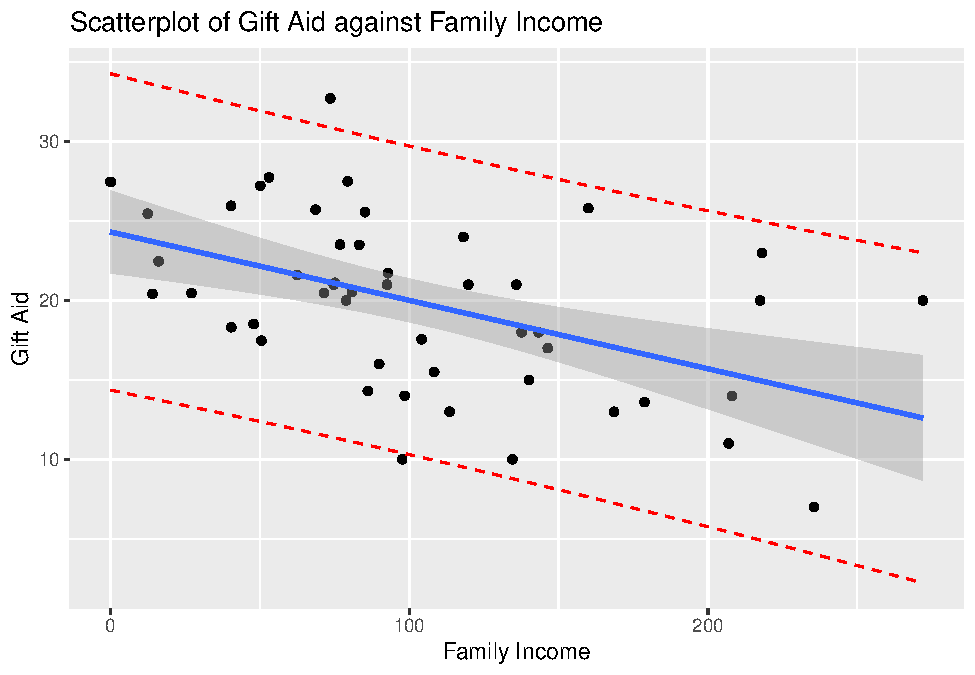
\includegraphics{bookdown-demo_files/figure-latex/unnamed-chunk-43-1.pdf}

As mentioned in the notes, the CI captures the location of the regression line, whereas the PI captures the data points.

  \bibliography{book.bib,packages.bib}

\end{document}
